\lstdefinestyle{MethodenListe}{
    language   = Python,
    numbers    = none,
    belowskip  = 0.25em,
    basicstyle = \tt\small
}

\lstdefinestyle{MethodenListeKlein}{
    language   = Python,
    numbers    = none,
    belowskip  = 0.25em,
    basicstyle = \tt\footnotesize
}

%%% Folie
\begin{frame}{Leitfragen des heutigen Kapitels}
    \begin{block}{Hardwareschaltungen mit Strom versorgen}
        \begin{itemize}
            \footnotesize
            \setlength\itemsep{.5em}

            \item Was ist Strom und welche Begriffe muss ich kennen?
            \item Wie viel Strom benötigt mein Microcontroller-Board?
            \item Wie lange hält die Batterie bzw. der Akku?
            \item Was kostet der jährliche Stromverbrauch?
        \end{itemize}
    \end{block}

    \begin{block}{Signale verarbeiten und erzeugen}
        \begin{itemize}
            \footnotesize
            \setlength\itemsep{.5em}

            \item Welche Arten der Signalübertragung gibt es?
            \item Welche Signalarten kann mein Microcontroller verarbeiten?
            \item Wie werden Sensoren/Aktoren mit dem Microcontroller verbunden?
            \item Wie lassen sich Hardwareschäden dabei vermeiden?
            \item Wie lassen sich inkompatible Logikpegel anpassen?
        \end{itemize}
    \end{block}

    \begin{block}{Mechanische Arbeit verrichten}
        \begin{itemize}
            \footnotesize
            \setlength\itemsep{.5em}

            \item Wie viel Strom kann mein Microcontroller-Board bereitstellen?
            \item Wie können stärkere Lastströme geschaltet werden?
        \end{itemize}
    \end{block}
\end{frame}

%%% Folie
\begin{frame}{Lernziele}
    \begin{block}{Physikalische Grundlagen}
        \begin{itemize}
            \footnotesize
            \setlength\itemsep{.5em}

            \item Eine einfache Definition des elektrischen Stroms kennen und verstehen
            \item Die Begriffe ,,Spannung'', ,,Stromstärke'' und ,,Widerstand''' erklären
            \item Die Unterschiede zwischen ,,Gleichstrom'' und ,,Wechselstrom'' kennen
            \item Das Ohmsche Gesetz anwenden können
        \end{itemize}
    \end{block}

    \begin{block}{Stromversorgung für eingebettete Systeme}
        \begin{itemize}
            \footnotesize
            \setlength\itemsep{.5em}

            \item Die Anforderungen typischer Microcontroller an die Stromversorgung kennen
            \item Die Funktionsweise eines einfachen USB-Trafonetzteils verstehen
            \item Die Lebensdauer einer Batterie/Akku abschätzen können
            \item Den Verbrauch und die erwarteten Stromkosten berechnen können
        \end{itemize}
    \end{block}

    \begin{block}{Sensoren und Aktoren}
        \begin{itemize}
            \footnotesize
            \setlength\itemsep{.5em}

            \item Die gängigen Schnittstellen eingebetteter Systeme erklären können
            \item Die Hardwareschnittstellen zumindest grundlegend programmieren können
            \item Analoge und digitale Sensoren und Aktoren verbinden können
            \item Stromstärken und Spannungen für den Microcontroller anpassen
        \end{itemize}
    \end{block}
\end{frame}

%-------------------------------------------------------------------------------
\section{Physikalische Grundlagen}
%-------------------------------------------------------------------------------

%%% Folie
\begin{frame}[allowframebreaks]{Was ist elektrischer Strom?}
    \begin{columns}
        \footnotesize

        \column{.6\textwidth}
        \raisebox{-0.5\height}{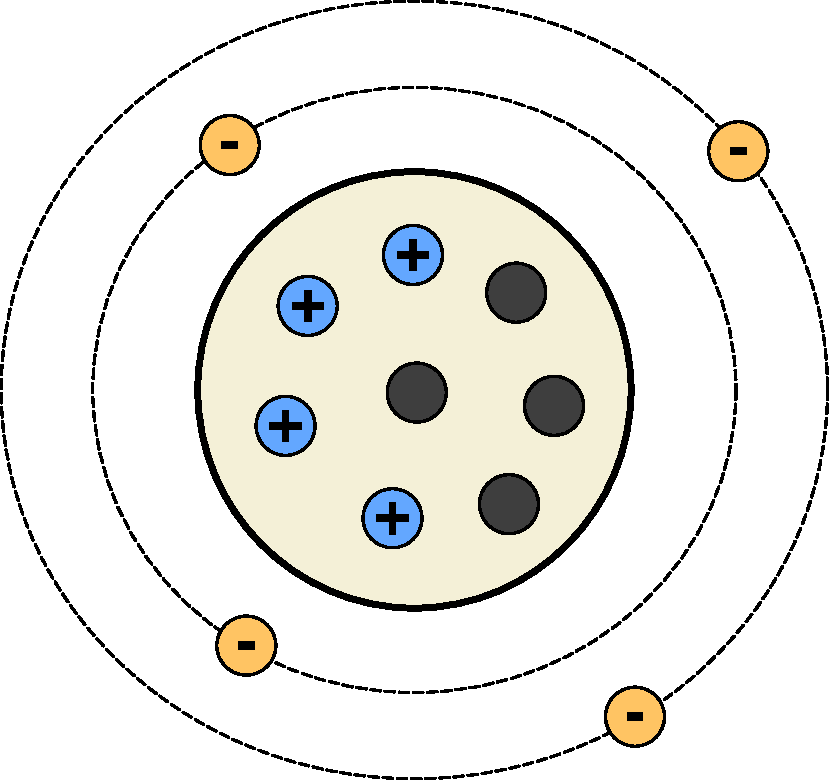
\includegraphics[width=.6\textwidth]{img/atom_detail}}

        \column{.4\textwidth}
        \raisebox{-0.25\height}{
\includegraphics[width=.4cm]{img/atom_kern}}
        \hskip 1em
        Atomkern \\
        \smallskip

        \raisebox{-0.25\height}{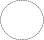
\includegraphics[width=.4cm]{img/atom_schale}}
        \hskip 1em
        Schale \\
        \bigskip

        \raisebox{-0.25\height}{
\includegraphics[width=.4cm]{img/atom_elektron}}
        \hskip 1em
        Elektron \\
        \smallskip

        \raisebox{-0.25\height}{
\includegraphics[width=.4cm]{img/atom_proton}}
        \hskip 1em
        Proton \\
        \smallskip

        \raisebox{-0.25\height}{
\includegraphics[width=.4cm]{img/atom_neutron}}
        \hskip 1em
        Neutron \\
    \end{columns}

    \bigskip
    \bigskip

    \parbox{\linewidth}{
        \scriptsize
        Am einfachsten lässt sich die Wirkungsweise des elektrischen Stroms verstehen,
        wenn man das alte Bohrsche Atommodell betrachtet, bei dem jedes Atom in Analogie
        an unser Sonnensystem als ein Kern mit Protonen und Neutronen mit diese umkreisenden
        Elektronen beschrieben wird.
        \smallskip

        Damit Strom in einem Material fließen kann, muss ein Teil der darin enthaltenen
        Elektronen mit geringem Energieaufwand frei beweglich sein. Man spricht dann von
        einem \textbf{Leiter}. Beispielsweise besitzen alle Metalle ein freies Elektron
        auf der äußersten Hülle, das leicht vom Atomkern gelöst werden kann.
        \smallskip

        In nicht-leitenden Materialien -- sog. \textbf{Isolatoren} -- gibt es keine frei
        beweglichen Elektronen, so dass ein großer Kraftaufwand zum Herauslösen benötigt
        wird. In \textbf{Halbleitern} kann die Anzahl der freien Elektronen während der
        Herstellung oder später durch äußere Umstände beeinflusst werden.
    }

    %%% Folie
    \framebreak

    \begin{columns}
        \column{\dimexpr\paperwidth-28pt}
        \begin{center}
            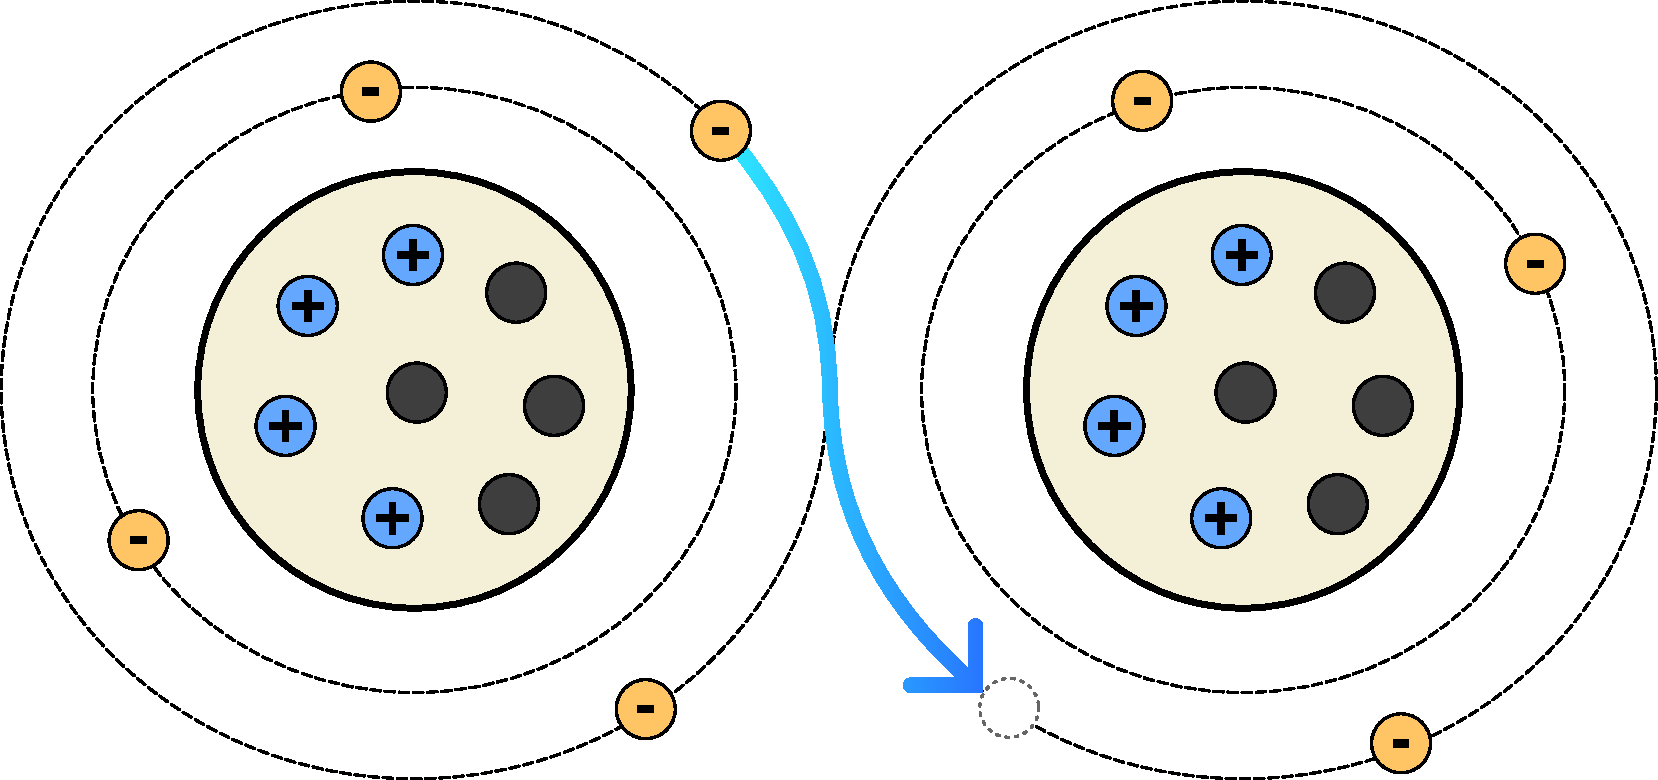
\includegraphics[width=.7\textwidth]{img/atom_elektronenfluss}
        \end{center}
    \end{columns}

    \bigskip

    \parbox{\linewidth}{
        \scriptsize
        Im Normalzustand sind die meisten Atome elektrisch neutral, da sie die
        gleiche Anzahl Protonen wie Elektronen besitzen. Atome mit einem Überschuss
        oder Mangel an Elektronen werden \textbf{Ionen} genannt und sind
        \textbf{elektrisch geladen}. Wurde beispielsweise ein Elektron aus der
        äußeren Hülle eines Atoms heraus gelöst, kann ein benachbartes Elektron
        überspringen, wodurch Strom fließt.
        \smallskip

        \textbf{Elektrischer Strom} entspricht somit der \textbf{Bewegung freier
        Elektronen} innerhalb eines leitfähigen Materials. Strom entsteht, indem
        die freien Elektronen \textbf{durch magnetische oder chemische Einwirkung}
        in Bewegung versetzt werden. Allerdings darf man das nicht nicht so vorstellen,
        dass ein Elektron geradlinig durch das Material hindurch wandert. Viel mehr
        nimmt es einen zufälligen Weg und schiebt dabei wie eine Billardkugel die
        umliegenden Elektronen aus dem Weg, da sich Elementarteilchen mit gleicher
        Ladung immer abstoßen.
    }

    %%% Folie
    \framebreak

    \parbox{\linewidth}{
        \footnotesize
        Folgende Begriffe sind zur Beschreibung elektrischer Ströme von besonderer Bedeutung:
    }

    \begin{block}{Spannung \hfill (Voltage)}
        \smallskip
        \parbox{\linewidth}{
            \scriptsize

            Die Spannung wird immer \textbf{zwischen zwei Punkten} gemessen und beschreibt
            wie viele Elektronen auf der einen Seite zu viel oder auf der anderen Seite zu
            wenig sind. Sie beschreibt somit die \textbf{Ladungsdifferenz} (Potentialunterschied)
            zwischen den beiden Punkten und wird in der Einheit \textbf{Volt} gemessen.
            Sie liefert die Kraft, die auf die Elektronen ausgeübt wird, um sie in Bewegung
            zu setzen und ist, sofern die beiden Punkte über ein elektrisch leitendes Material
            verbunden sind, die \textbf{Ursache für den Stromfluss}.
        }
    \end{block}

    \begin{block}{Masse \hfill (Ground)}
        \smallskip
        \parbox{\linewidth}{
            \scriptsize

            Beschreibt in einem Stromkreis den gemeinsamen Bezugspunkt, vom dem aus die meisten
            anderen Spannungen gemessen werden. Entspricht bei einer Batterie dem Minuspol oder
            beim Hausstrom dem Neutralleiter. In einem Stromkreis fließt der Strom gedanklich
            immer zur Masse.
        }
    \end{block}

    \begin{block}{Stromstärke \hfill (Current)}
        \smallskip
        \parbox{\linewidth}{
            \scriptsize

            Die Stromstärke gibt an, wie viele Elektronen innerhalb einer gegebenen Zeit einen
            Punkt passieren. Es handelt sich sozusagen um die \textbf{Geschwindigkeit}, mit
            der sich die Elektronen durch den Leiter bewegen. Je mehr Elektronen innerhalb einer
            Zeitspanne durch den Leiter wandern, desto mehr Strom fließt. Die Stromstärke wird
            in der Einheit \textbf{Ampere} gemessen.
        }
    \end{block}

    \begin{block}{Widerstand \hfill (Resistance)}
        \smallskip
        \parbox{\linewidth}{
            \scriptsize

            Jedes Bauteil in einem Stromkreis besitzt einen impliziten Widerstand, der den
            \textbf{Elektronenfluss hindert}, indem ein Teil der Energie in \textbf{Wärme
            oder Strahlung} umgewandelt wird. Ein Widerstand reduziert somit die Stromstärke
            und wird in der Einheit \textbf{Ohm} gemessen. Man kann ihn sich wie einen Knick
            in einem Wasserschlauch vorstellen, durch den nur noch wenig Wasser gelangt,
            obwohl das Wasser mit starker Kraft hinein gedrückt wird.
        }
    \end{block}
\end{frame}

%%% Folie
\begin{frame}{Maßeinheiten und Größen}
    \begin{tabularx}{\textwidth}{|X|X|X|}
        \hline
        \textbf{Präfix} & \textbf{Zehnerpotenz} & \textbf{Dezimalwert} \\
        \hline

        Mega & $10^6$ & 1.000.000 \\
        \hline

        Kilo & $10^3$ & 1.000 \\
        \hline

        -- & $10^0$ & 1 \\
        \hline

        Milli & $10^{-3}$ & 0,001 \\
        \hline

        Mikro & $10^{-6}$ & 0,000.001 \\
        \hline

        Nano & $10^{-9}$ & 0,000.000.001 \\
        \hline

        Piko & $10^{-12}$ & 0,000.000.000.001 \\
        \hline
    \end{tabularx}

    \bigskip
    \bigskip
    \bigskip

    {
        \small

        \textbf{Spannung:} Volt \hskip 1em
        \textbf{Stromstärke:} Ampere \hskip 1em
        \textbf{Widerstand:} Ohm \hskip 1em
        \textbf{Leistung:} Watt
    }
\end{frame}

%%% Folie
\begin{frame}{Schaltpläne zur Dokumentation von Stromkreisen}
    \begin{center}
        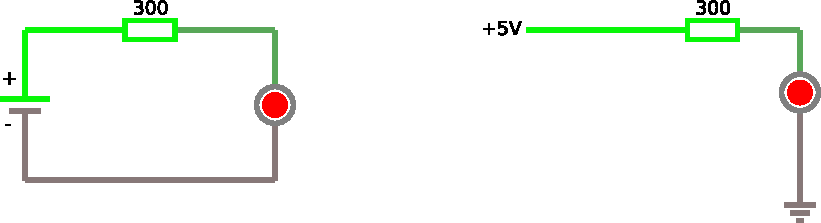
\includegraphics[width=\textwidth]{img/mini-stromkreis}
    \end{center}

    \hfill%
    \CircuitJS{https://www.falstad.com/circuit/circuitjs.html?ctz=CQAgjCAMB0l3BWcMBMcUHYMGZIA4UA2ATmIxAUgoqoQFMBaMMAKADcQ9CAWCwqrr248ooytSqToCFgCdOI4bzCQUQkVVyQWAd2Rq+AkQn5QWYQin3rlq3iapWAJnQBmAQwCuAGwAuDbzoncFEpSFYAJXA1PBAlcAtY+Mk42lCoaTlo7iSRMGxTZJAtc0twAqp4-NMEbl5nNy8-AKCQlJhwlgBzcpq63toMQlCWAA9ObmI40k4EKcorZSsAHQAHMdmIBBRYvAQkBGwIJZAGFiA}
    \bigskip

    \parbox{\linewidth}{
        \scriptsize

        Elektrische Schaltungen werden immer als \textbf{Stromkreis} entworfen
        und in einem \textbf{Schaltplan} dokumentiert. Gedanklich fließt der
        Strom in diesem vom Pluspol zum Minuspol (linke, meist in Schulbüchern
        anzutreffende Darstellung) bzw. vom Pluspol der Spannungsquelle zur Masse
        (rechte Darstellung). Tatsächlich beruht diese Annahme aber auf einem Irrtum,
        weil es die negativ geladenen Elektronen sind, die sich vom Minus- zum
        Pluspol bewegen. Da sich dadurch aber nur das Vorzeichen in den Berechnungen
        ändert, wurde die Konvention unter dem Namen \textbf{technische Stromrichtung}
        in Abgrenzung zur \textbf{tatsächlichen Stromrichtung} beibehalten.
        \smallskip

        Die Symbole in den obigen Schaltplänen haben folgende Bedeutung:
        \smallskip

        \begin{center}
            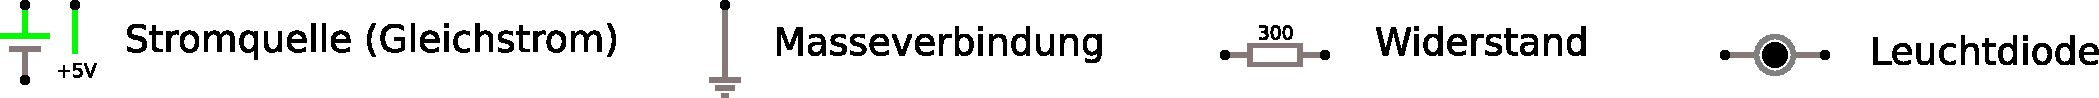
\includegraphics[width=\textwidth]{img/schaltsymbole}
        \end{center}
    }
\end{frame}

%%% Folie
\begin{frame}[allowframebreaks]{Das Ohmsche Gesetz}
    \begin{columns}
        \column{.4\textwidth}
        \begin{center}
            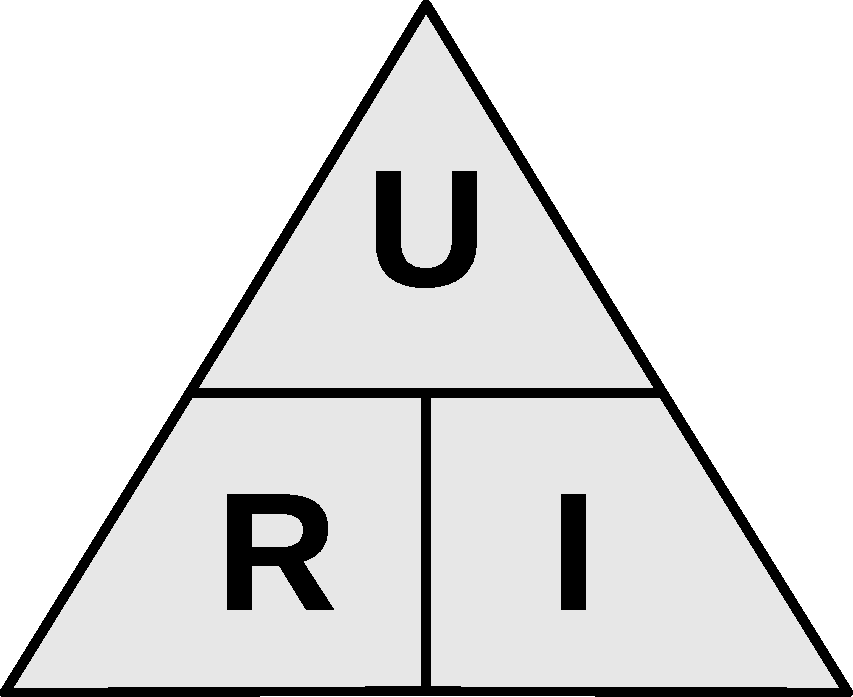
\includegraphics[width=.4\textwidth]{img/formel_uri}
        \end{center}

        \medskip

        \begin{tabular}{ccll}
            $U$ & = & $R \times I$ & {\scriptsize Spannung in Volt} \\
            $R$ & = & $U / I$ & {\scriptsize Widerstand in Ohm} \\
            $I$ & = & $U / R$ & {\scriptsize Stromstärke in Ampere}\\
        \end{tabular}

        \column{0.6\textwidth}
        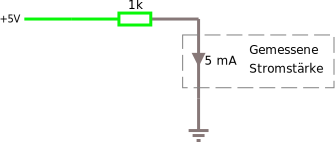
\includegraphics[width=\textwidth]{img/ohmsches-gesetz-schaltplan}

        \hfill%
        \CircuitJS{https://www.falstad.com/circuit/circuitjs.html?ctz=CQAgjCAMB0l3BWcMBMcUHYMGZIA4UA2ATmIxAUgoqoQFMBaMMAKACURiAWLkbQvCDx4q-QVSpdaUGTAQsATpx58ByDClXjkcFtgxUwkDVvWaegiBJYBzMyAv2uI2SwAe4MCmwPIP5sQ+UoQO4JoA4nQAtnQAzrF0AHZ07p7eDiiaASFcKEi8XiAAygAuCgD2UbElACcKANYpAEbICCHYeAVoglz6UCxAA}
    \end{columns}

    \bigskip

    \Justified{
        \scriptsize

        Die \textbf{Spannung} einer Stromquelle sorgt dafür, dass sich die Elektronen in
        Bewegung setzen und ein Strom fließt, wenn zwischen beiden Polen eine elektrische
        Verbindung hergestellt wird. Die dabei entstehende \textbf{Stromstärke} hängt
        vom \textbf{Widerstand} aller durchlaufenen Bauteile (und dem Innenwiderstand
        der Stromquelle) ab. In bestimmten Fällen kann ein linearer Zusammenhang entsprechend
        der Formel $I = U / R$ angenommen werden, so dass mit zwei bekannten Werten
        der dritte errechnet werden kann.
        \smallskip

        Für uns ist dies besonders wichtig, um die maximale Stromstärke zu begrenzen,
        die der Microcontroller an ein angeschlossenes Bauteil abgibt, um sowohl den
        Microcontroller als auch das Bauteil vor Beschädigungen zu schützen. Beispiele
        für typische Fragestellungen sind:

        \begin{itemize}
            \item Welche Stromstärke fließt durch eine Schaltung (wie viel Strom ,,zieht`` die Schaltung)?
            \item Welcher Widerstand wird benötigt, um eine bestimmte Stromstärke zu erhalten?
            \item Liegt die Stromstärke innerhalb der erlaubten Grenzen für den Microcontroller und das Bauteil?
        \end{itemize}
    }

    \framebreak

    \textcolor{gray}{
        \tiny
        \textbf{Kennlinie:} Stromstärke (Y-Achse) in Abhängigkeit zur Spannung (X-Achse), der Widerstand entspricht der Tangentensteigung
    }
    {
        \footnotesize

        \begin{columns}
            \column{.33\textwidth}
            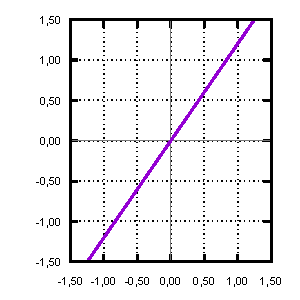
\includegraphics[width=\textwidth]{img/kennlinie-widerstand} \\
            \smallskip
            \hfill \textbf{Widerstand} \hfill%
            \raisebox{-0.4\height}{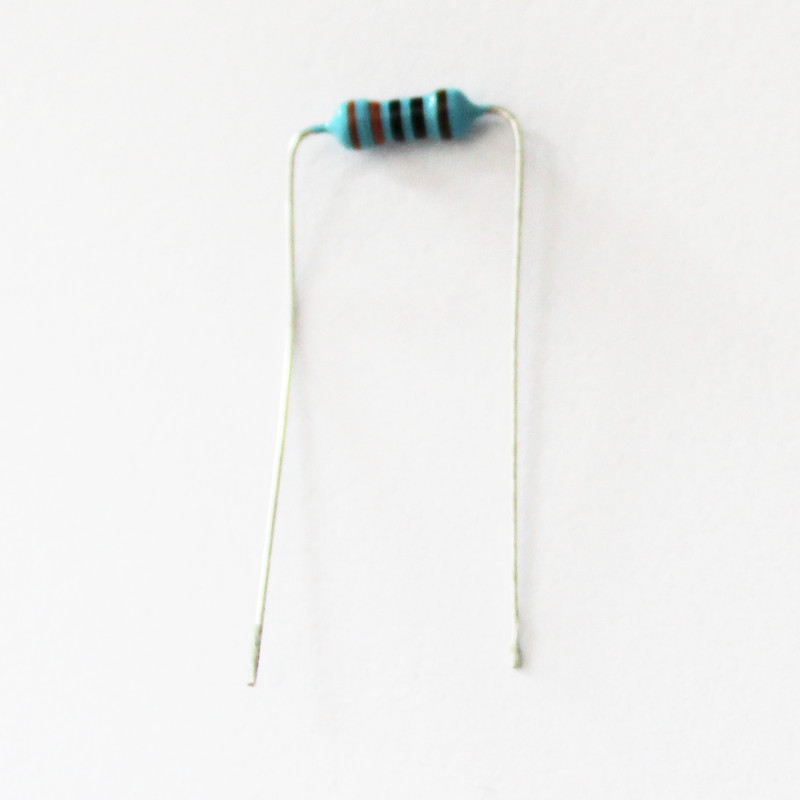
\includegraphics[width=2.5em]{img/komponenten_elementar_widerstand}}

            \column{.33\textwidth}
            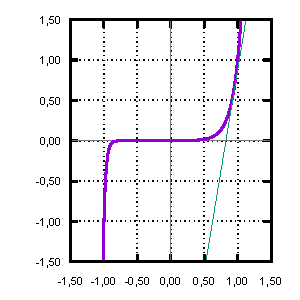
\includegraphics[width=\textwidth]{img/kennlinie-diode} \\
            \smallskip
            \hfill \textbf{Leuchtdiode} \hfill%
            \raisebox{-0.4\height}{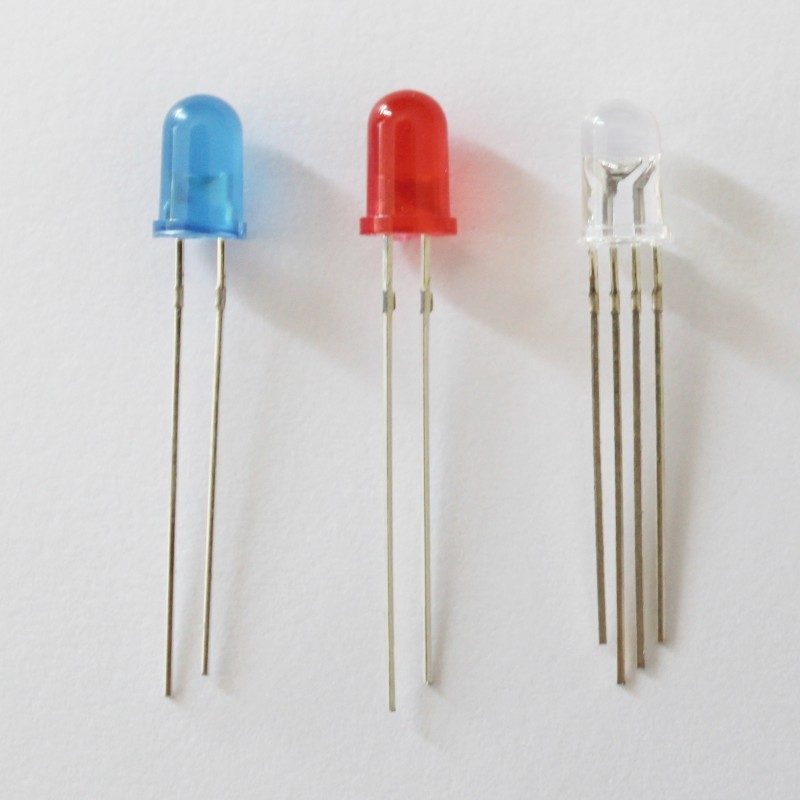
\includegraphics[width=2.5em]{img/komponenten_elementar_led}}

            \column{.33\textwidth}
            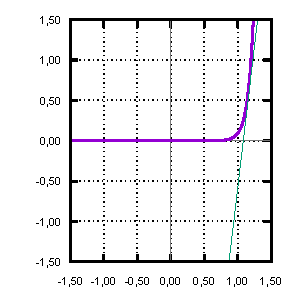
\includegraphics[width=\textwidth]{img/kennlinie-transistor} \\
            \smallskip
            \hfill \textbf{npn-Transistor} \hfill%
            \raisebox{-0.4\height}{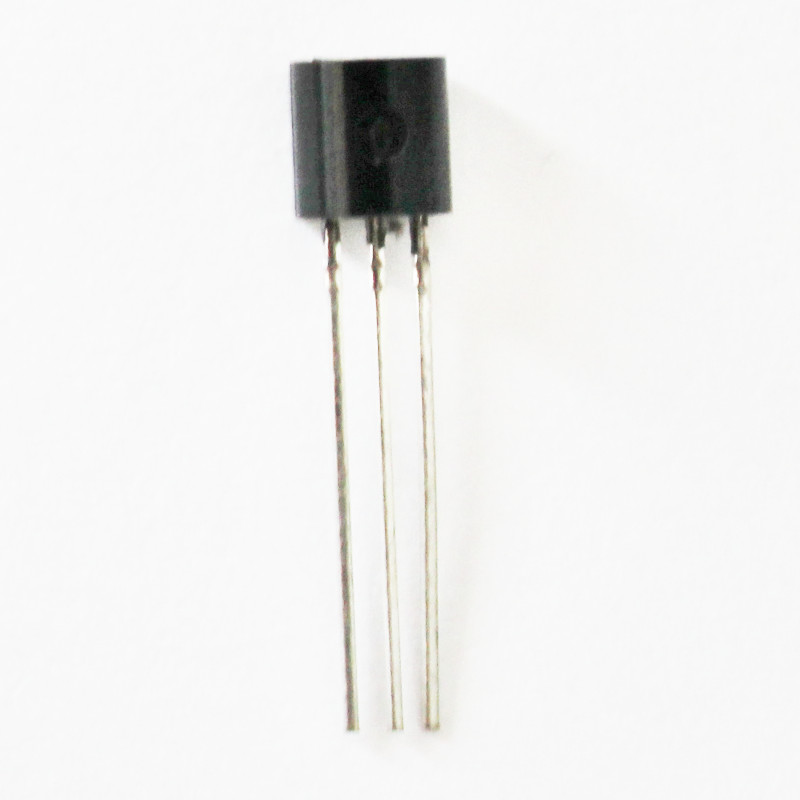
\includegraphics[width=2.5em]{img/komponenten_elementar_transistor}}
        \end{columns}
    }
    \bigskip

    \Justified{
        \tiny

        Das Ohmsche Gesetz gilt nur für \textbf{ideale Widerstände}, die deshalb auch
        \textbf{ohmsche Widerstände} genannt werden. Genau genommen besagt es, dass
        der Widerstand solcher Bauteile für jede Spannung derselbe ist und sich die
        Stromstärke daher linear zur Spannung verhält. In unserem Fall handelt es sich
        dabei um kleine Keramikwiderstände, die wir in unsere Schaltungen einbauen
        (Abbildung links).
        \smallskip

        Insbesondere Bauteile auf Halbleiterbasis besitzen jedoch eine \textbf{nicht-lineare Kennlinie},
        so dass die durchfließende Stromstärke nicht linear von der Spannung abhängt. Der Widerstand
        dieser Bauteile ergibt sich ebenfalls aus Spannung und Stromstärke, besitzt aber keinen konstanten
        Wert. In Anlehnung an das Ohmsche Gesetz kann er näherungsweise als \textbf{differentieller
        Widerstand} $r = \Delta U / \Delta I$ am gewählten Arbeitspunkt berechnet werden (sog. Kleinsignalverhalten).
    }
\end{frame}

%%% Folie
\begin{frame}{Berechnung der Leistung}
    \begin{columns}
        \column{.2\textwidth}
        \begin{center}
            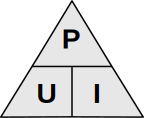
\includegraphics[width=.9\textwidth]{img/formel_pui}
        \end{center}

        \column{.4\textwidth}
        \hfill%
        \begin{tabular}{ccll}
            $P$ & = & $U \times I$ & {\scriptsize Leistung in Watt} \\
            $U$ & = & $P / I$ & {\scriptsize Spannung in Volt} \\
            $I$ & = & $P / U$ & {\scriptsize Stromstärke in Ampere}\\
        \end{tabular}
        \hfill%

        \column{.4\textwidth}
        {
            \scriptsize
            \hfill%
            $Leistung = \frac{Energie\:innerhalb\:Zeit}{Zeit}$
        }
    \end{columns}

    \vskip 1cm

    \Justified{
        \scriptsize
        Ein weiterer, gelegentlich anzutreffender Begriff ist die in \textbf{Watt}
        gemessene \textbf{Leistung}, welche die innerhalb einer Zeitspanne umgesetzte
        Energie geteilt durch die Zeitspanne beschreibt. Die Überlegung ist analog
        zur Geschwindigkeit (Weg durch Zeit), nur das keine Wegstrecke überbrückt,
        sondern Energie übertragen wird.
        \smallskip

        Ihre elektrische Definition lautet $P = U \times I$, so dass ein Watt der Leistung
        entspricht, die benötigt wird, um an einem \textbf{ohmschen Widerstand von einem
        Ohm eine Spannung von einem Volt} (und damit eine Stromstärke von einem Ampere)
        \textbf{während einer Sekunde} zu erhalten. Daraus folgt, dass sich die Leistung
        aus dem Produkt der beiden anderen Werte \textit{Spannung} und \textit{Stromstärke}
        bildet, da die Stromstärke bereits stark vereinfacht als ,,Anzahl Elektronen je Sekunde''
        definiert ist.
        \smallskip

        Meist kommen wir damit nur in Berührung, wenn es um die \textbf{Nennleistung
        eines Netzteils} oder die damit verbundenen \textbf{Stromkosten} geht. Denn
        anstatt der maximal abgebbaren Stromstärke in Ampere geben die meisten Netzteile
        lediglich eine Maximalleistung in Watt an, die zunächst in Ampere umgerechnet werden muss.
        Typische Fragestellungen könnten dabei sein:
        \smallskip

        \begin{itemize}
            \item Wie viel Leistung steht zum Verrichten anderer Arbeiten zur Verfügung?
            \item Welche maximale Stromstärke kann mein Netzteil bereitstellen?
            \item Wie hoch sind die Stromkosten für die beanspruchte Leistung?
        \end{itemize}
    }
\end{frame}

%-------------------------------------------------------------------------------
\section{Stromversorgung}
%-------------------------------------------------------------------------------

%%% Folie
\begin{frame}{Gleichstrom vs. Wechselstrom}
    Grundsätzlich werden drei Arten von Strom unterschieden:
    \medskip

    \begin{block}{Gleichstrom}
        \smallskip
        \parbox{\linewidth}{
            \footnotesize
            Besitzt eine zeitlich konstante Spannung \\
            \textbf{Beispiel:} Interne Stromversorgung eines Computers
        }
    \end{block}

    \begin{block}{Wechselstrom}
        \smallskip
        \parbox{\linewidth}{
            \footnotesize
            Die Spannung ist variabel und ändert regelmäßig die Richtung \\
            \textbf{Beispiel:} Netzstrom, bipolares Analogsignal, Audiosignale
        }
    \end{block}

    \begin{block}{Mischstrom}
        \smallskip
        \parbox{\linewidth}{
            \footnotesize
            Ist mathematisch eine Überlagerung von Gleich- und Wechselströmen \\
            \textbf{Beispiel:} Analoge Sensorsignale, unipolares Analogsignal
        }
    \end{block}

    \bigskip

    \begin{columns}
        \column{.33\textwidth}
        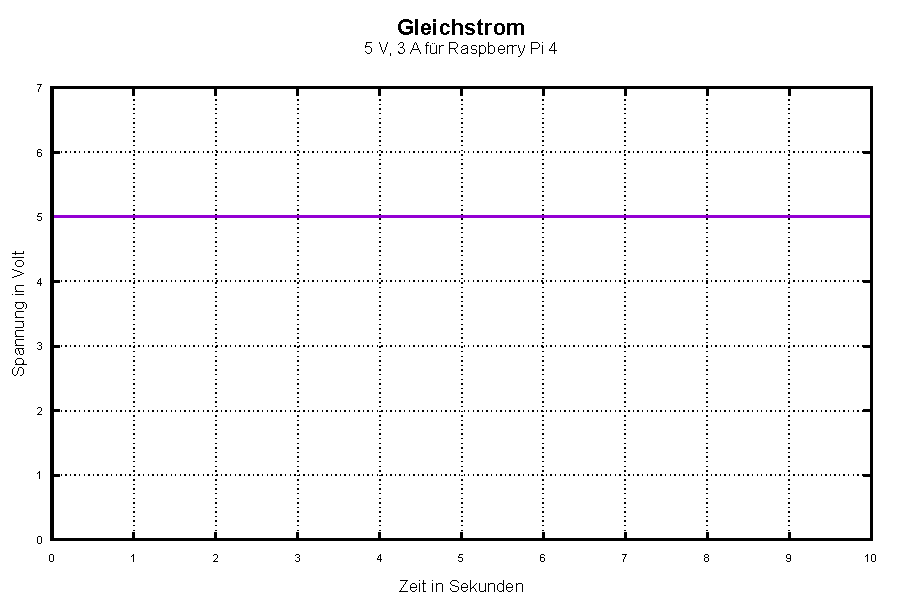
\includegraphics[width=\textwidth]{img/strom-gleichstrom}

        \column{.33\textwidth}
        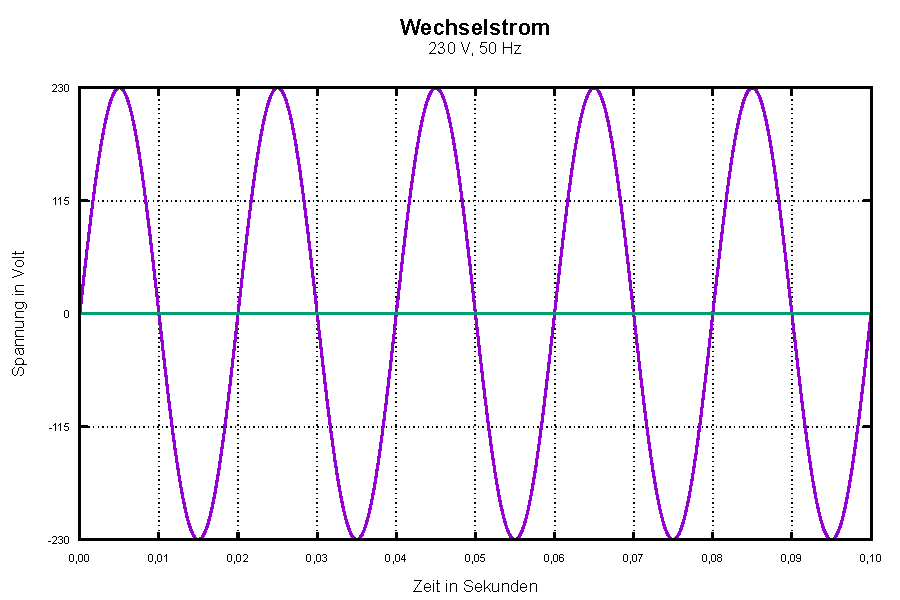
\includegraphics[width=\textwidth]{img/strom-wechselstrom}

        \column{.33\textwidth}
        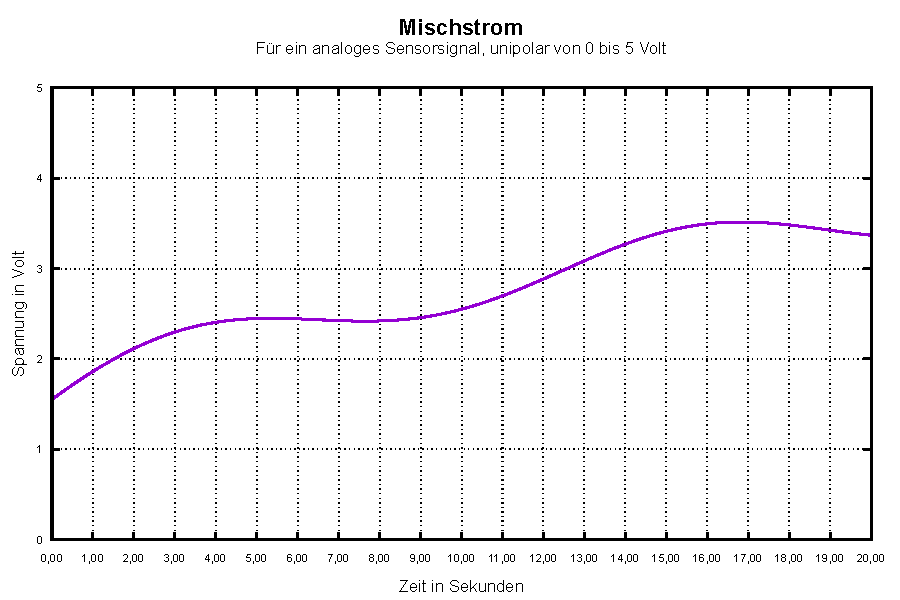
\includegraphics[width=\textwidth]{img/strom-analogsensor}
    \end{columns}
\end{frame}

%%% Folie
{
\scriptsize

\begin{frame}{Stromversorgung für eingebettete Systeme}
    \begin{columns}
        \column{.5\textwidth}
        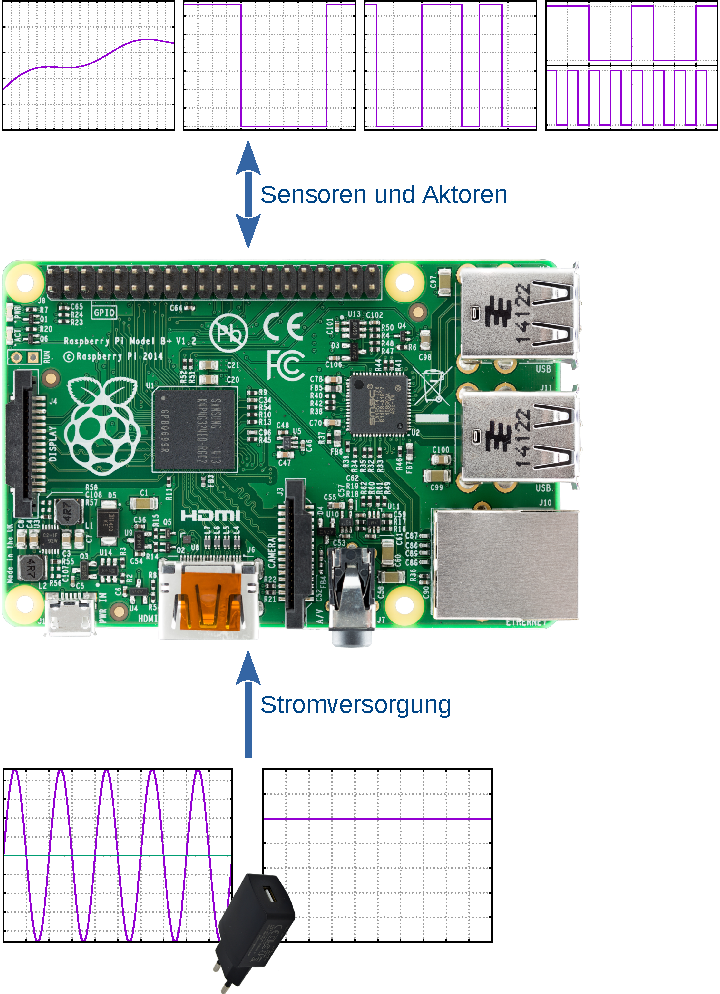
\includegraphics[width=\textwidth]{img/raspi-stromarten}

        \column{.5\textwidth}

        \begin{block}{Stromversorgung}
            \smallskip
            \parbox{\linewidth}{
                Das Stromnetz liefert Wechselstrom mit 230\,V und 16\,A.
                Der Raspberry Pi benötigt aber \textbf{5\,V Gleichstrom und $\pm$ 3\,A}.
                Ein Arduino Uno benötigt zum Vergleich \textbf{6-20\,V Gleichstrom}
                (wird intern auf 5\,V geregelt) und \textbf{$\geq$ 250\,mA}).
                \smallskip

                Das Netzteil muss daher den die Spannung reduzieren und den Strom gleichrichten.
                Eine mobile Stromversorgung muss mindestens genauso viel Strom liefern.
                \smallskip

                \textcolor{red}{
                    Die Spannung muss dabei möglichst konstant sein und darf nicht
                    überschritten werden, um Beschädigungen zu vermeiden!
                }
            }
        \end{block}

        \vfill

        \begin{block}{Batterielaufzeit}
            \smallskip
            \parbox{\linewidth}{
                Kann über die Nennladung der Batterie abgeschätzt werden, wenn diese
                bekannt ist:
                \smallskip

                $\text{Laufzeit in Stunden} = \frac{\text{Nennladung in Ah}}{\text{Stromverbrauch in A}}$
            }
        \end{block}

        \vfill

        \begin{block}{Stromkosten}
            \smallskip
            \parbox{\linewidth}{
                Kann durch Umrechnen des Stromverbrauchs in Killowatt berechnet werden:
                \smallskip

                $\text{Kosten} = \frac{5\,V \times 3\,A}{1000} \times \text{Stunden} \times \text{Strompreis je kWh}$
            }
        \end{block}
    \end{columns}
\end{frame}
}

%-------------------------------------------------------------------------------
\section{Signale verarbeiten und erzeugen}
%-------------------------------------------------------------------------------

%%% Folie
{
    \setbeamertemplate{background canvas}{
        \includegraphics[height=\paperheight, width=\paperwidth]{img/bauteile}
    }

    \begin{frame}[plain]
    \end{frame}
}

%%% Folie
{
\small

\begin{frame}{Beispiel: Elementare Bauteile}
    \begin{columns}
        \column[b]{.25\textwidth}
        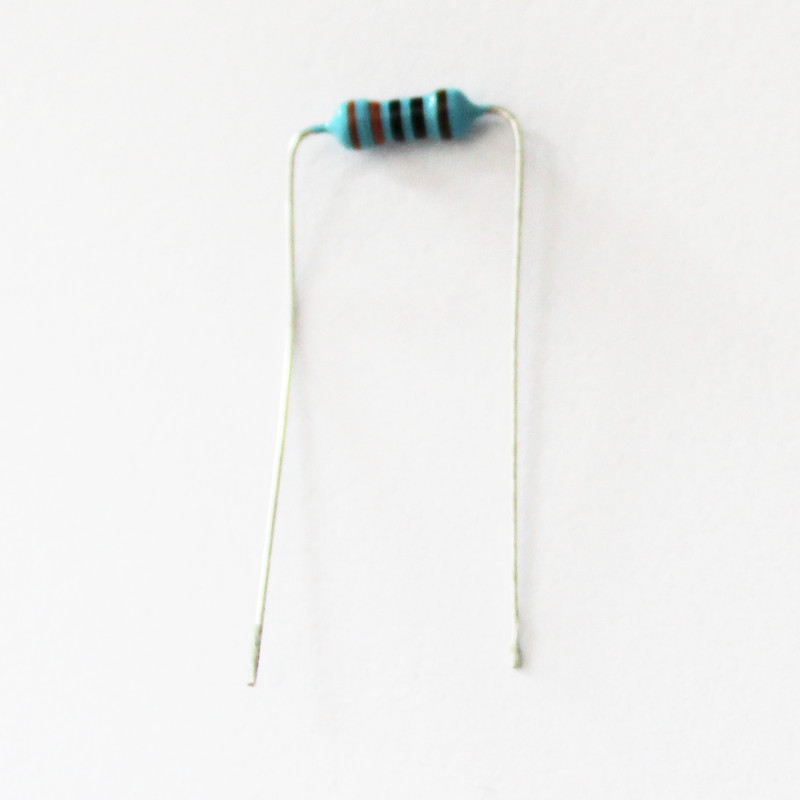
\includegraphics[width=.8\textwidth]{img/komponenten_elementar_widerstand} \\
        Widerstand

        \column[b]{.25\textwidth}
        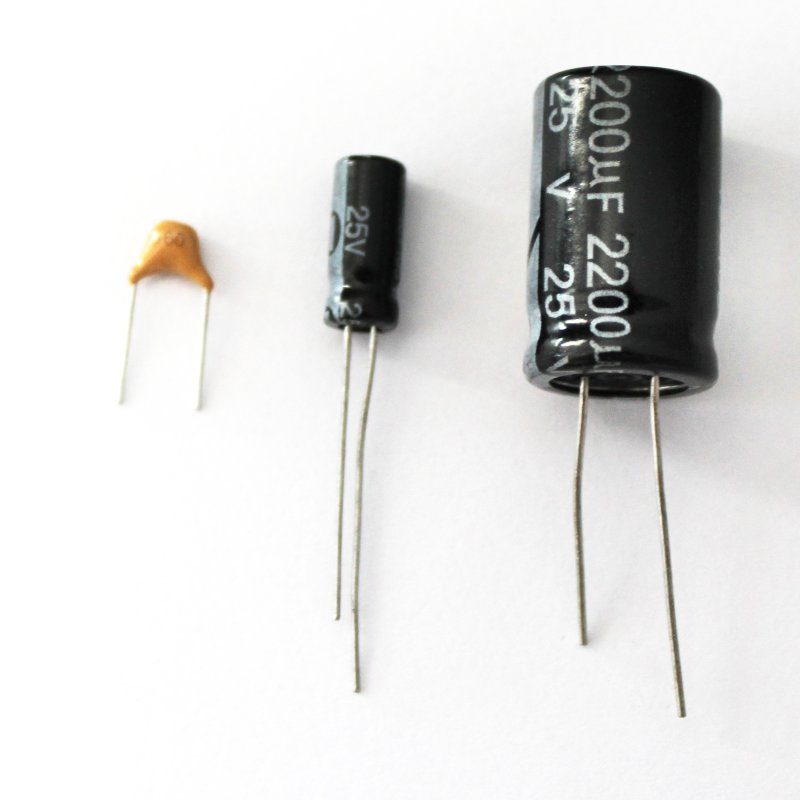
\includegraphics[width=.8\textwidth]{img/komponenten_elementar_kondensator} \\
        Kondensator

        \column[b]{.25\textwidth}
        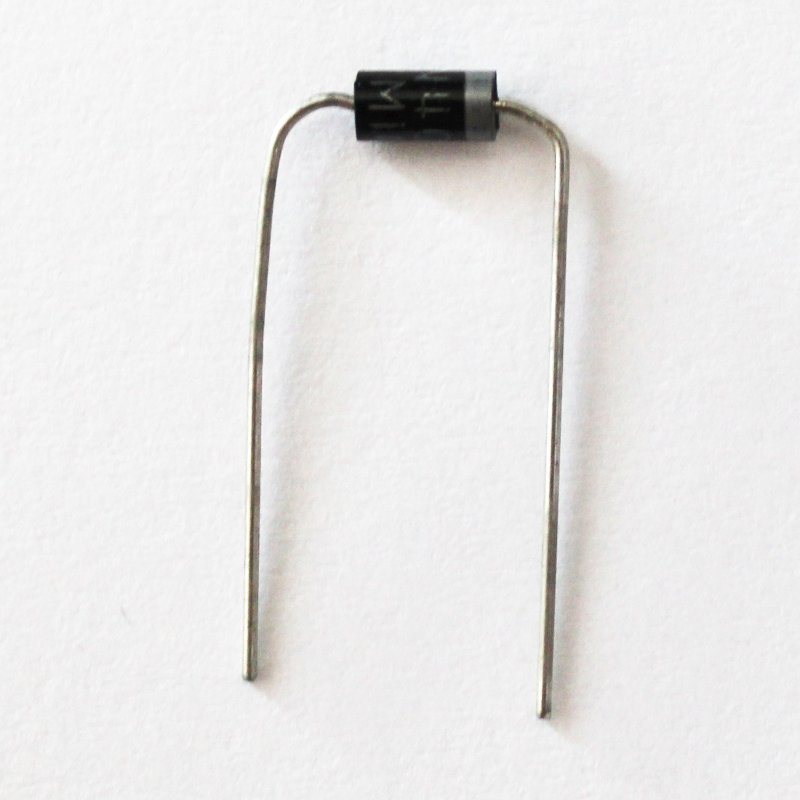
\includegraphics[width=.8\textwidth]{img/komponenten_elementar_diode} \\
        Diode

        \column[b]{.25\textwidth}
        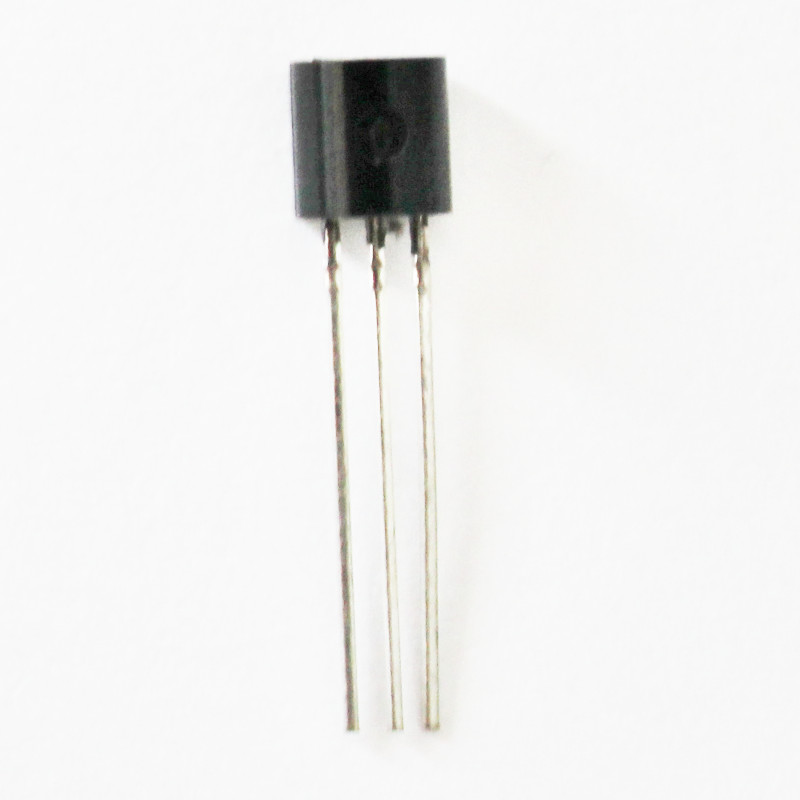
\includegraphics[width=.8\textwidth]{img/komponenten_elementar_transistor} \\
        Transistor
    \end{columns}

    \bigskip

    \begin{columns}
        \column[b]{.25\textwidth}
        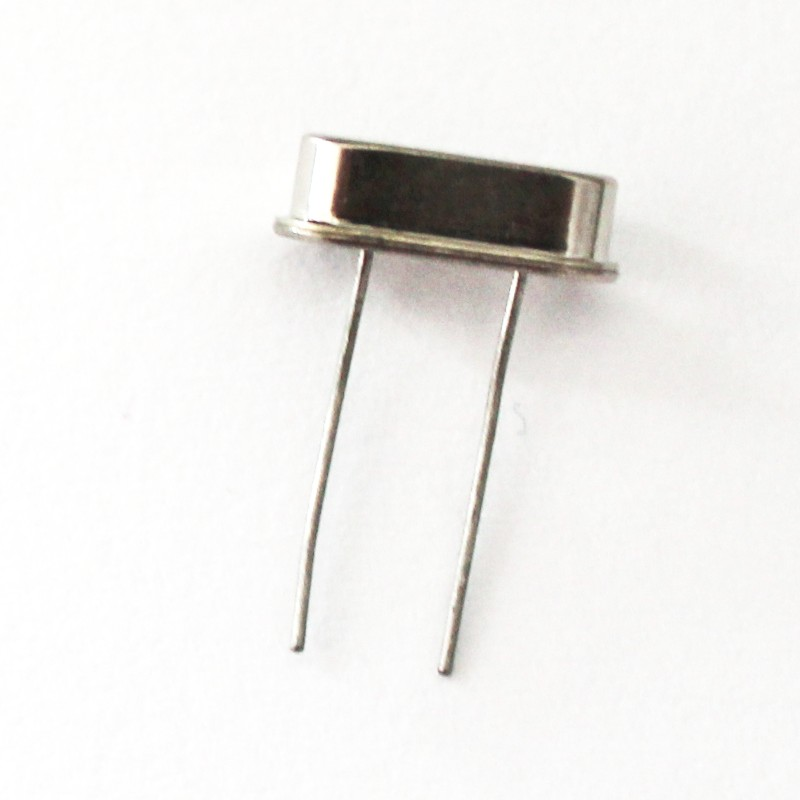
\includegraphics[width=.8\textwidth]{img/komponenten_elementar_quartz} \\
        Quartz-Kristal

        \column[b]{.25\textwidth}
        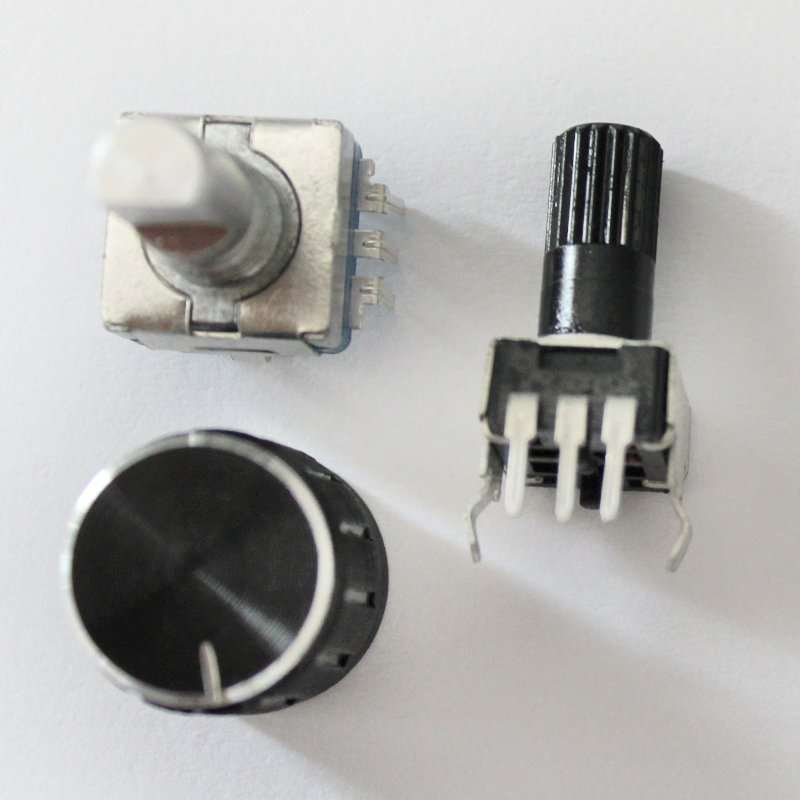
\includegraphics[width=.8\textwidth]{img/komponenten_elementar_drehregler} \\
        Drehregler

        \column[b]{.25\textwidth}
        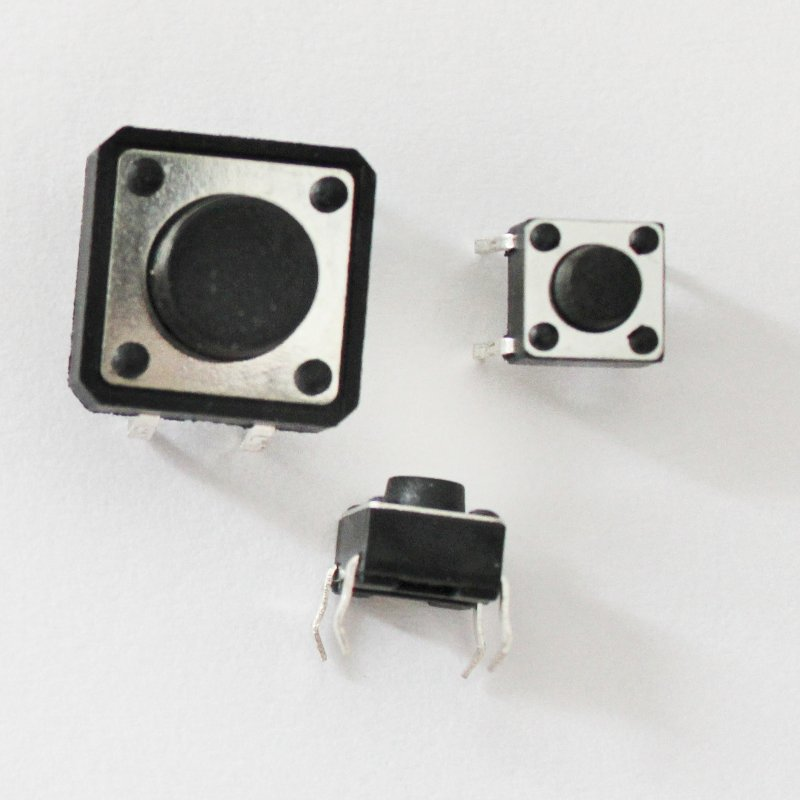
\includegraphics[width=.8\textwidth]{img/komponenten_elementar_taster} \\
        Taster, Schalter

        \column[b]{.25\textwidth}
        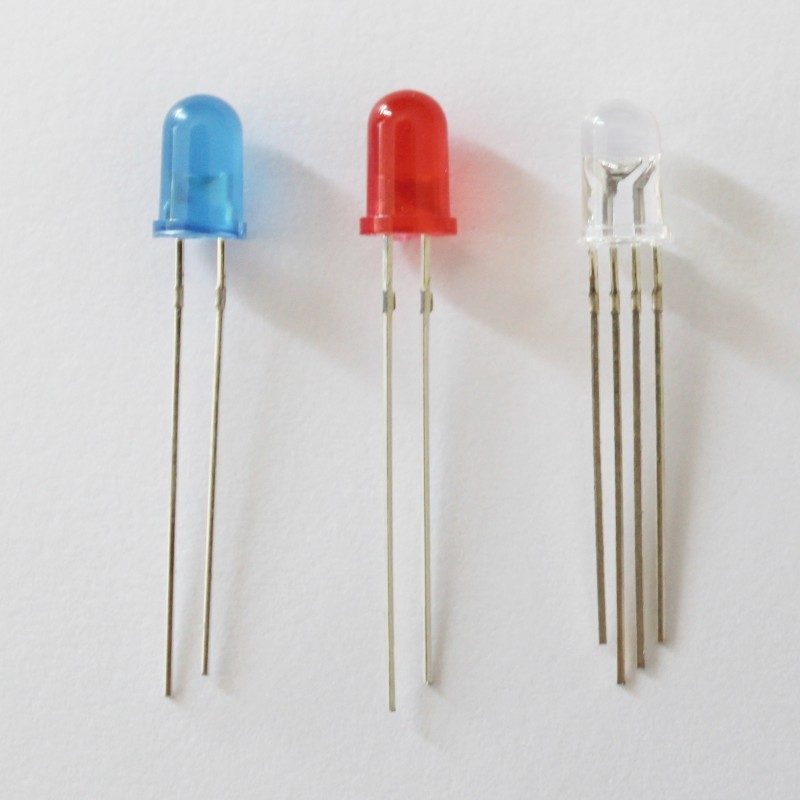
\includegraphics[width=.8\textwidth]{img/komponenten_elementar_led} \\
        Leuchtdiode
    \end{columns}
\end{frame}
}

%%% Folie
{
\small

\begin{frame}{Beispiel: Integrierte Schaltkreise}
    \begin{columns}
        \column[b]{.5\textwidth}
        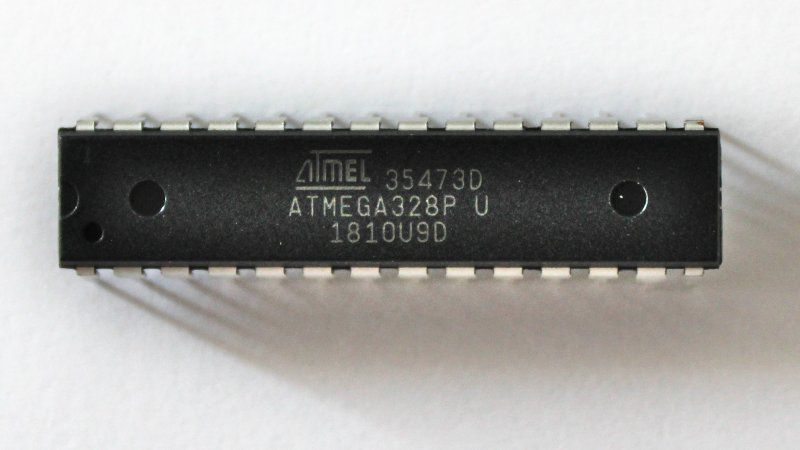
\includegraphics[width=.8\textwidth]{img/komponenten_ic_prozessor} \\
        Mikroprozessor, Mikrocontroller

        \column[b]{.5\textwidth}
        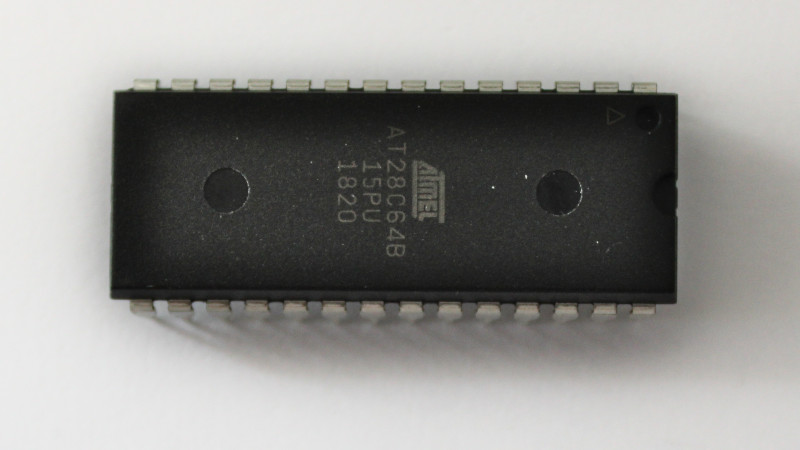
\includegraphics[width=.8\textwidth]{img/komponenten_ic_speicher} \\
        Speicherbaustein
    \end{columns}

    \bigskip

    \begin{columns}
        \column[b]{.5\textwidth}
        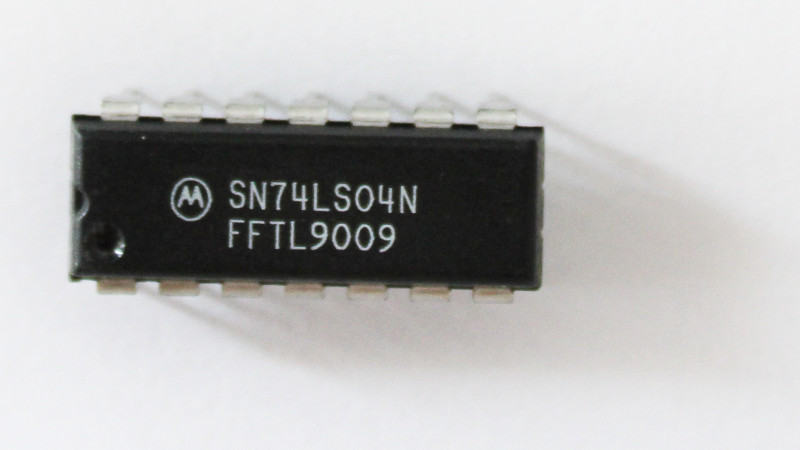
\includegraphics[width=.8\textwidth]{img/komponenten_ic_logikgatter} \\
        Logikbaustein (AND, OR, XOR, ...)

        \column[b]{.5\textwidth}
        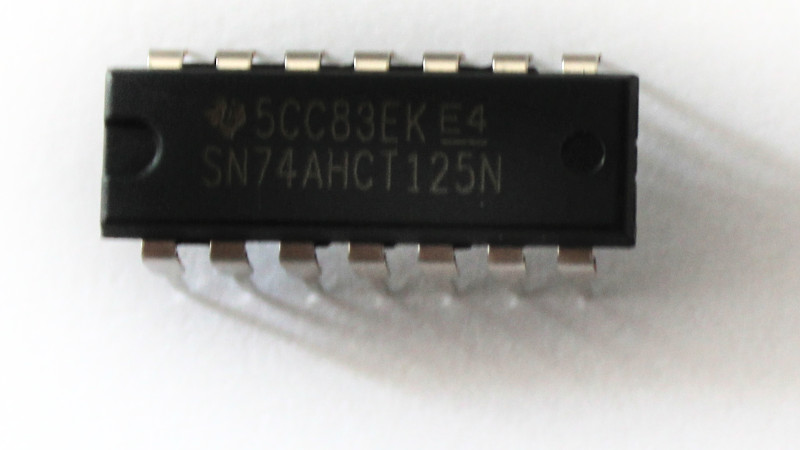
\includegraphics[width=.8\textwidth]{img/komponenten_ic_levelshifter} \\
        Level Shifter
    \end{columns}
\end{frame}
}

%%% Folie
{
\small

\begin{frame}{Beispiel: Vorgefertigte Baugruppen}
    \begin{columns}
        \column[b]{.5\textwidth}
        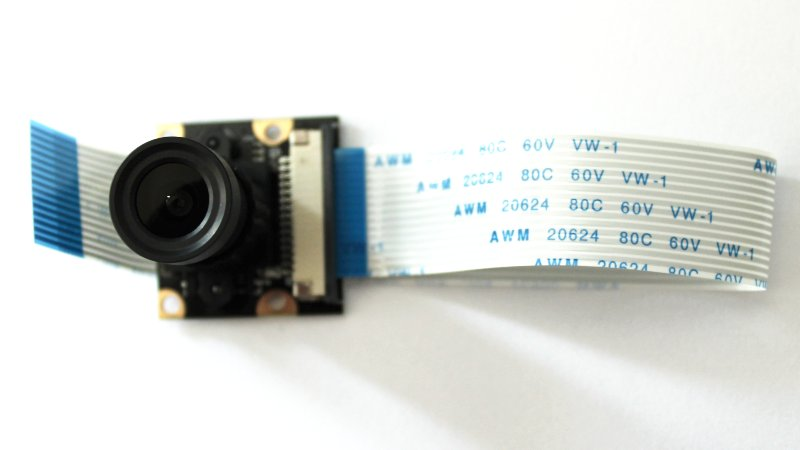
\includegraphics[width=.8\textwidth]{img/komponenten_baugruppen_kamera} \\
        Kameramodul

        \column[b]{.5\textwidth}
        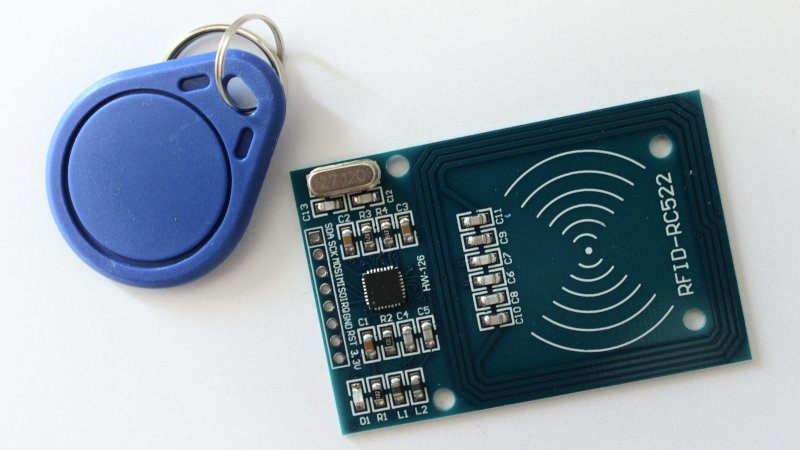
\includegraphics[width=.8\textwidth]{img/komponenten_baugruppen_rfid} \\
        RFID-Leser
    \end{columns}

    \bigskip

    \begin{columns}
        \column[b]{.5\textwidth}
        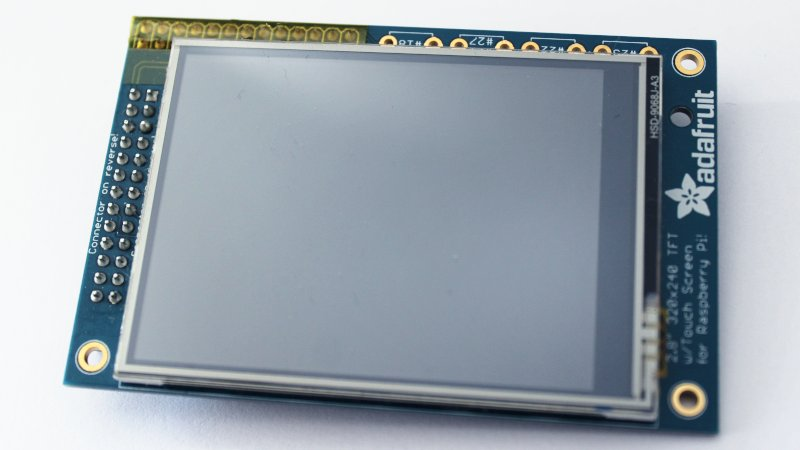
\includegraphics[width=.8\textwidth]{img/komponenten_baugruppen_display} \\
        Display

        \column[b]{.5\textwidth}
        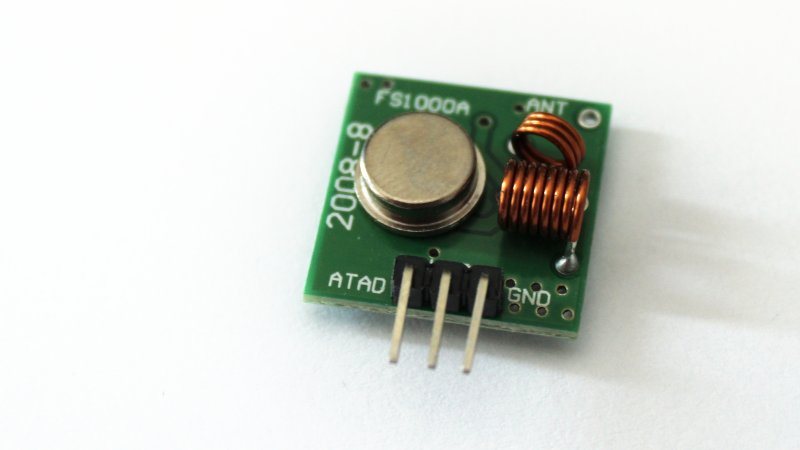
\includegraphics[width=.8\textwidth]{img/komponenten_baugruppen_funk} \\
        Funkmodul
    \end{columns}
\end{frame}
}

%%% Folie
{
\tiny

\begin{frame}[allowframebreaks]{Beispiel: Sensorkit aus der Vorlesung}
    \begin{columns}
        \column{\dimexpr\paperwidth-28pt}
        \begin{center}
            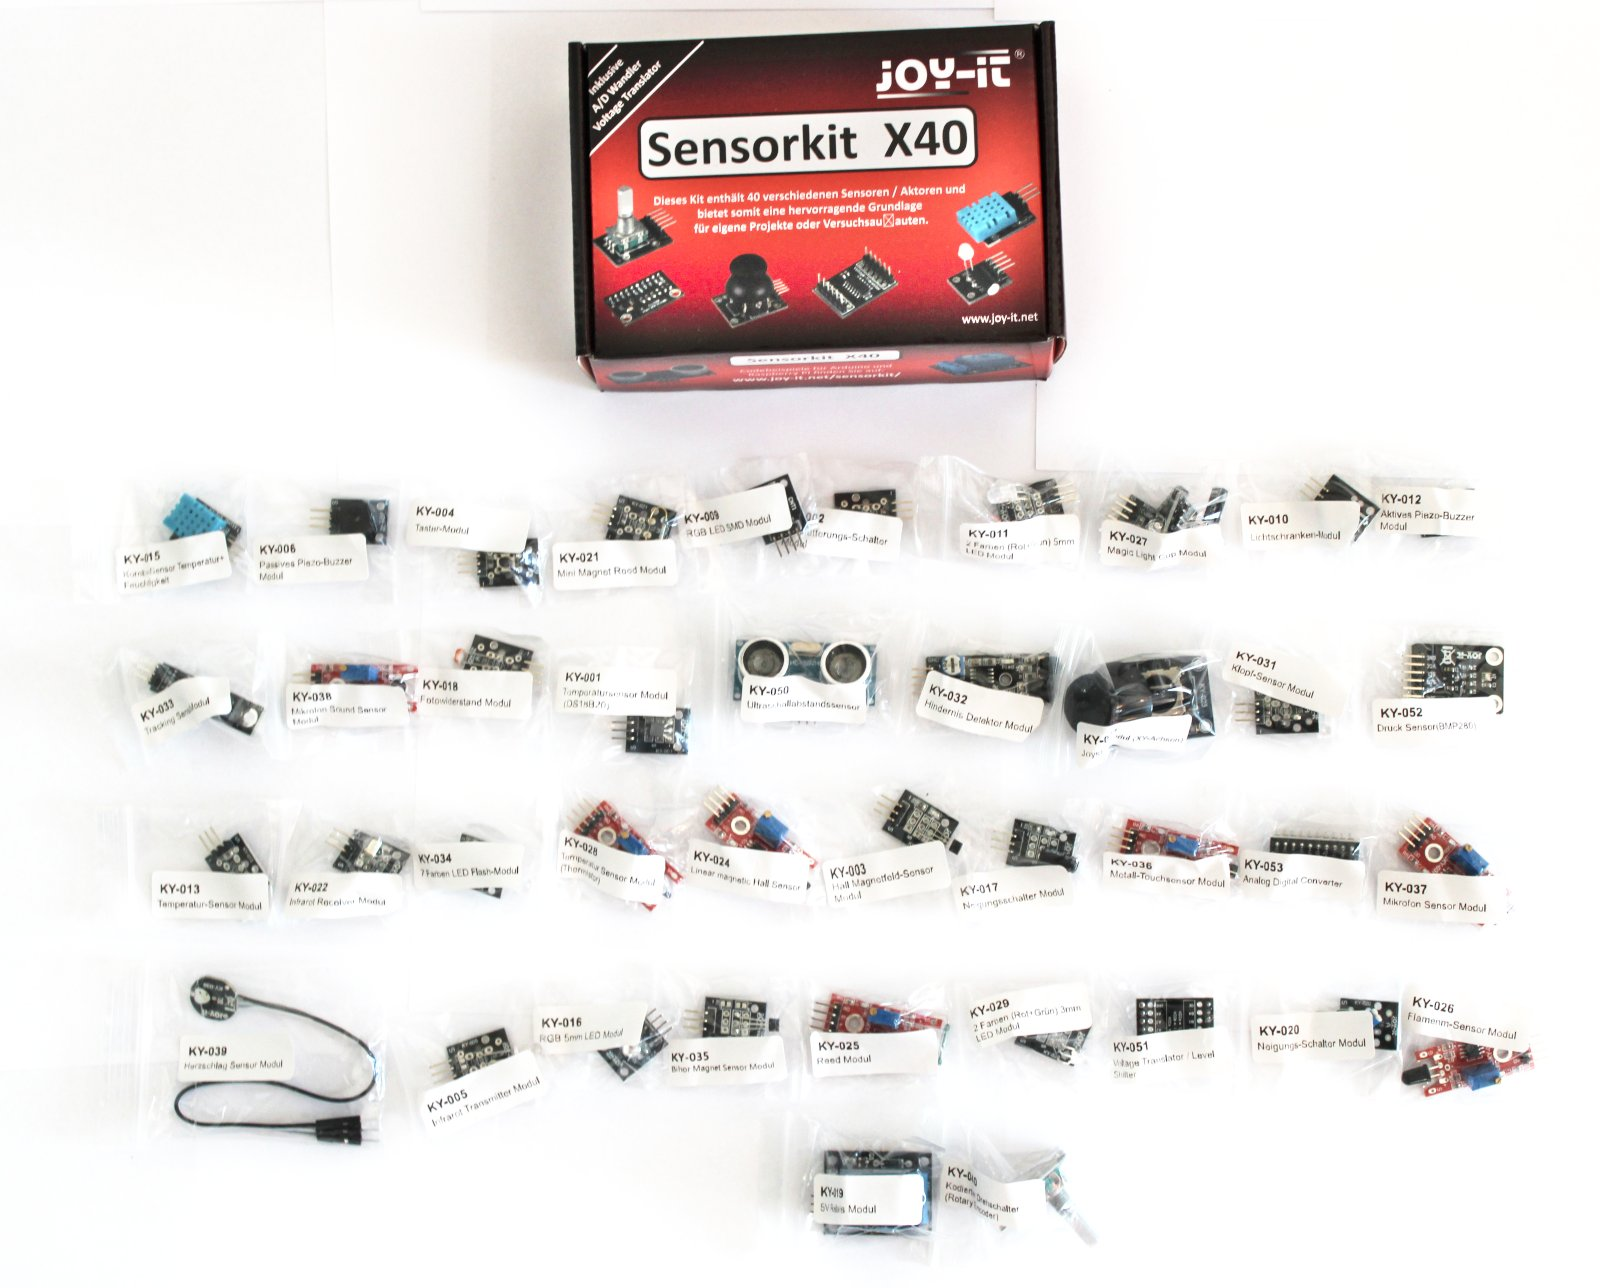
\includegraphics[height=.8\textheight]{img/sensorkit_alle}
        \end{center}
    \end{columns}

    \begin{block}{Umweltsensoren}
        \medskip
        \begin{columns}
            \column{0.5\textwidth}
            KY-001: Temperatursensor (DS18B20) \\
            KY-002: Erschütterungsschalter \\
            KY-003: Hall Magnetfeldsensor \\
            KY-010: Lichtschranke \\
            KY-013: Temperatursensor \\
            KY-015: Temperatur, Feuchtigkeit (DHT11) \\
            KY-017: Neigungsschalter \\
            KY-018: Fotowiderstand \\
            KY-020: Neigungsschalter \\
            KY-021: Mini Magnet-Reedkontakt \\
            KY-024: Linear Magnetic Hall-Sensor \\
            KY-025: Reedkontakt \\
            KY-026: Flammensensor \\

            \column{0.5\textwidth}
            KY-027: Magic Light Cup  \\
            KY-028: Temperatursensor (Thermistor) \\
            KY-031: Klopfsensor \\
            KY-032: Hindernisdetektor \\
            KY-033: Trackingsensor \\
            KY-035: Bihor Magnetsensor \\
            KY-036: Metall-Touchsensor \\
            KY-037: Mikrofon Soundsensor \\
            KY-038: Mikrofon Soundsensor \\
            KY-039: Herzschlagsensor \\
            KY-050: Ultraschallabstandssensor \\
            KY-052: Drucksensor (BMP280) \\
        \end{columns}
    \end{block}

    \begin{block}{Ein-/Ausgabemodule}
        \medskip
        \begin{columns}
            \column{0.5\textwidth}
            KY-004: Taster \\
            KY-022: Infrarot-Receiver \\
            KY-023: XY-Joystick \\
            KY-040: Kodierter Drehschalter (Rotary Encoder) \\
            \smallskip
            KY-005: Infrarot-Transmitter \\
            KY-006: Passiver Piezo-Buzzer \\
            KY-009: RGB-LED (Surface-Mount) \\

            \column{0.5\textwidth}
            KY-011: 2-Farben (Rot und Grün) LED \\
            KY-012: Aktiver Piezo-Buzzer \\
            KY-016: RGB-LED (Through-Hole) \\
            KY-019: 5V Relais \\
            KY-029: 2-Farben (Rot und Grün) LED \\
            KY-034: 7-Farben LED \\
        \end{columns}
    \end{block}

    \begin{block}{Hilfsbausteine}
        \medskip
        \begin{columns}
            \column{0.5\textwidth}
            KY-051: Voltage Translator / Level Shifter \\

            \column{0.5\textwidth}
            KY-053: Analog/Digital Converter \\
        \end{columns}
    \end{block}
\end{frame}
}

%%% Folie
{
\small

\begin{frame}{Beispiel: Modular einsetzbare Geräte}
    \begin{columns}
        \column[b]{.5\textwidth}
        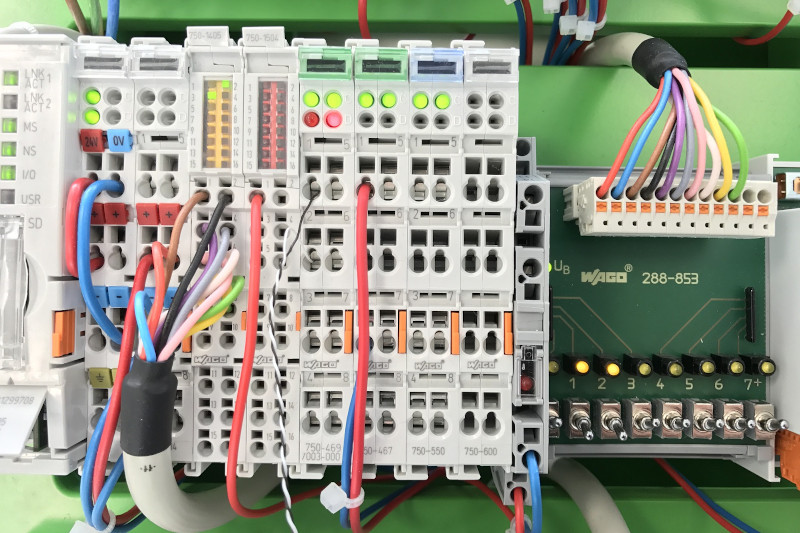
\includegraphics[width=.8\textwidth]{img/komponenten_geraete_industriesteuerung} \\
        Industrielle Steuergeräte

        \column[b]{.5\textwidth}
        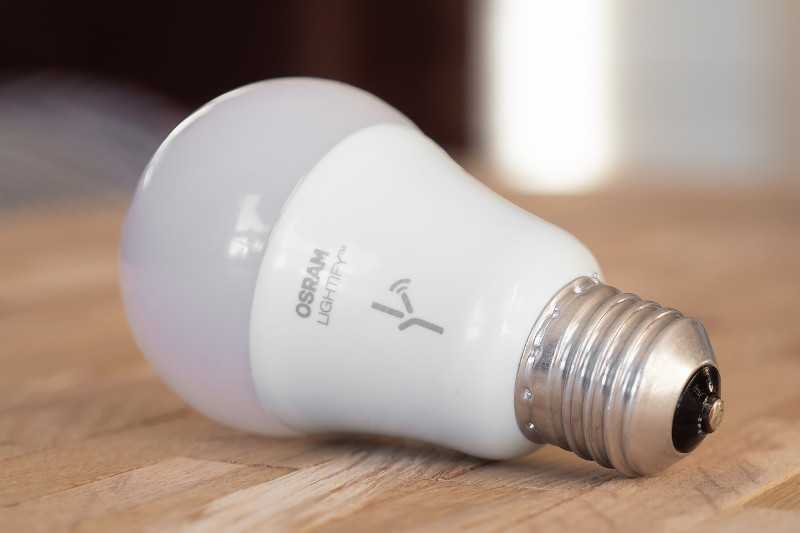
\includegraphics[width=.8\textwidth]{img/komponenten_geraete_smarthome} \\
        Smart-Home-Komponenten
    \end{columns}

    \bigskip

    \begin{columns}
        \column[b]{.5\textwidth}
        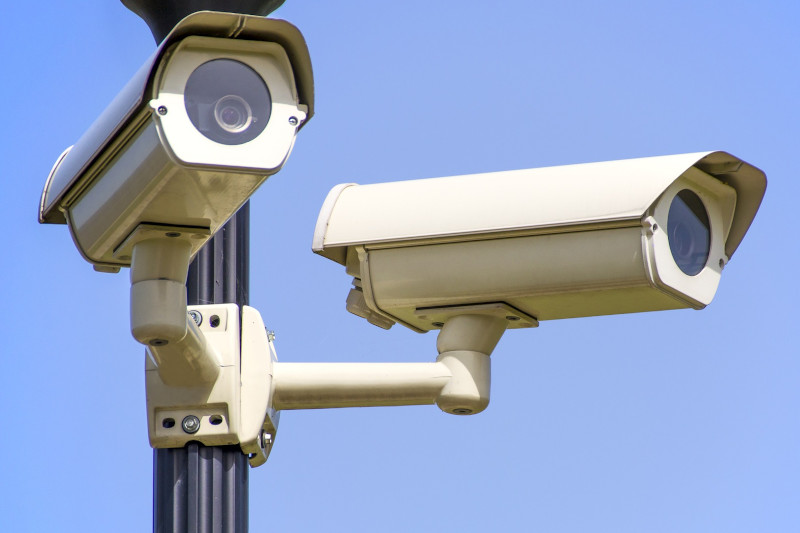
\includegraphics[width=.8\textwidth]{img/komponenten_geraete_ipkamera} \\
        IP-Kameras

        \column[b]{.5\textwidth}
        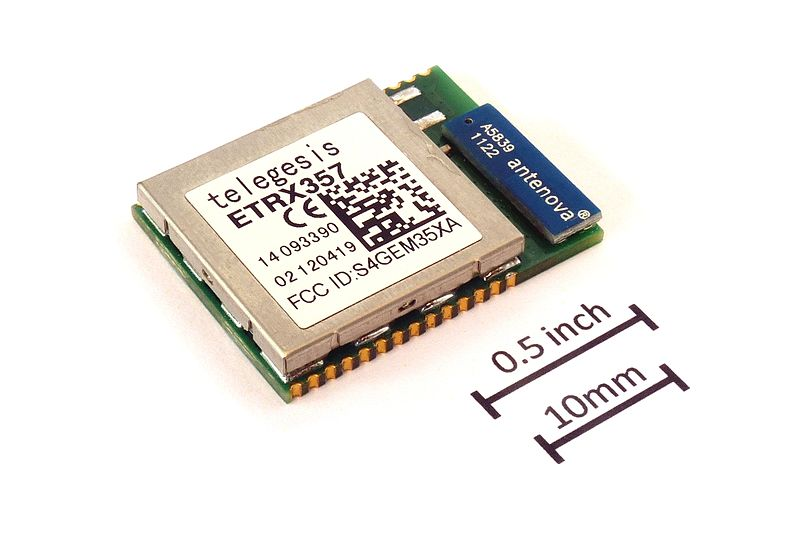
\includegraphics[width=.8\textwidth]{img/komponenten_geraete_zigbee} \\
        ZigBee-Sensoren und Aktoren
    \end{columns}
\end{frame}
}

%%% Folie
{
    \setbeamertemplate{background canvas}{
        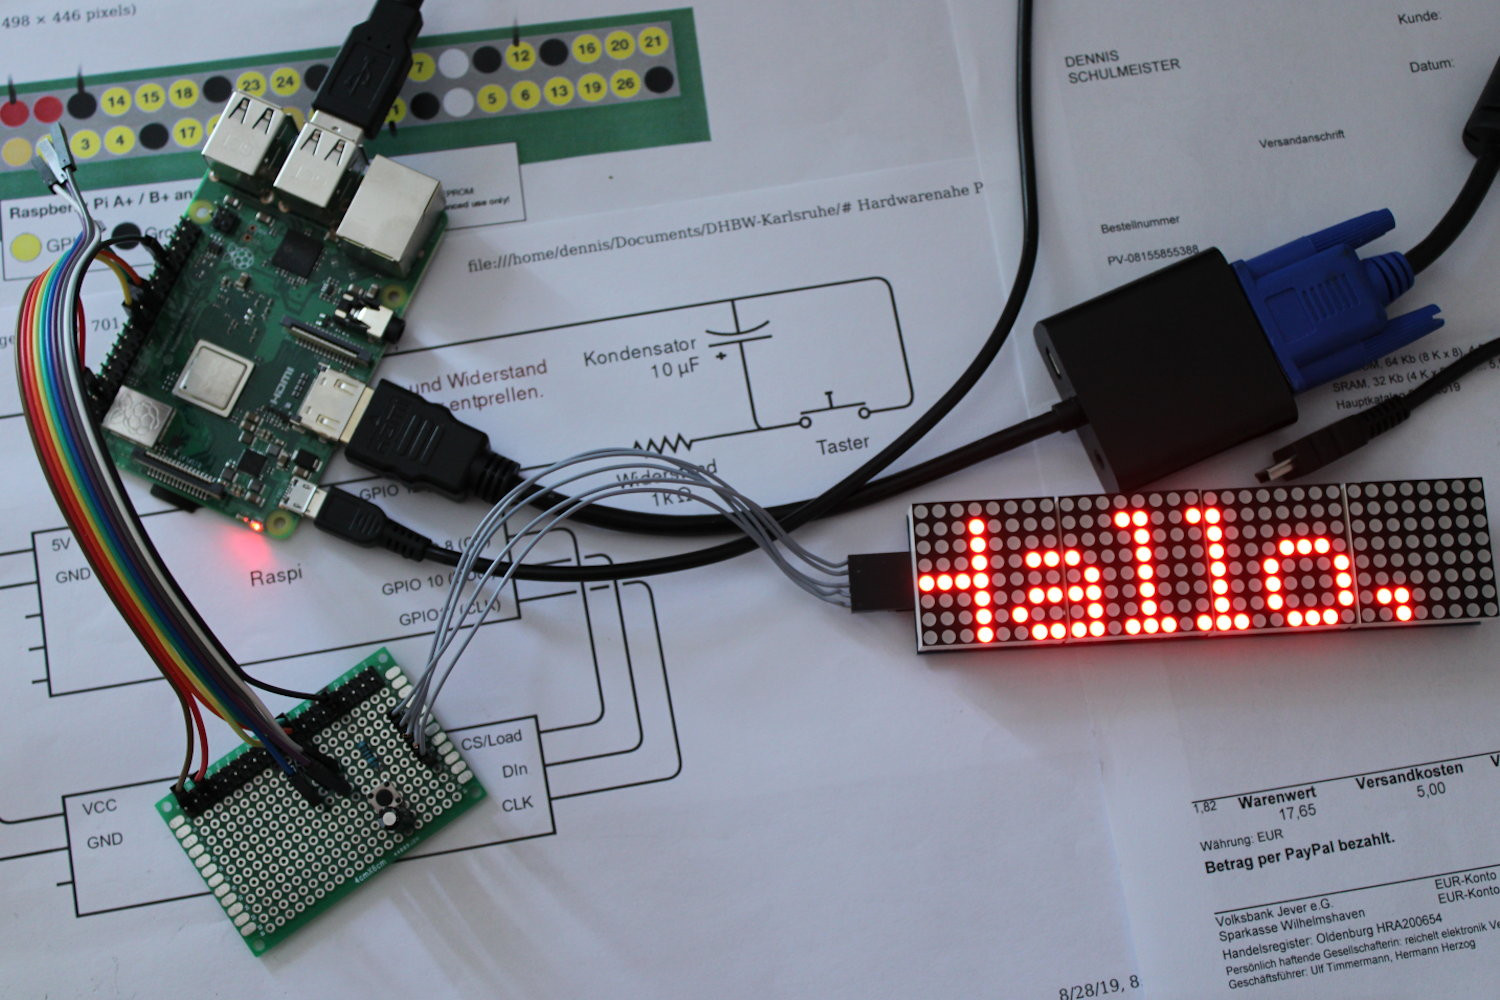
\includegraphics[height=\paperheight, width=\paperwidth]{img/vorgehen_lochrasterplatine}
    }

    \begin{frame}[plain]
    \end{frame}
}

%%% Folie
{
    \setbeamertemplate{background canvas}{
        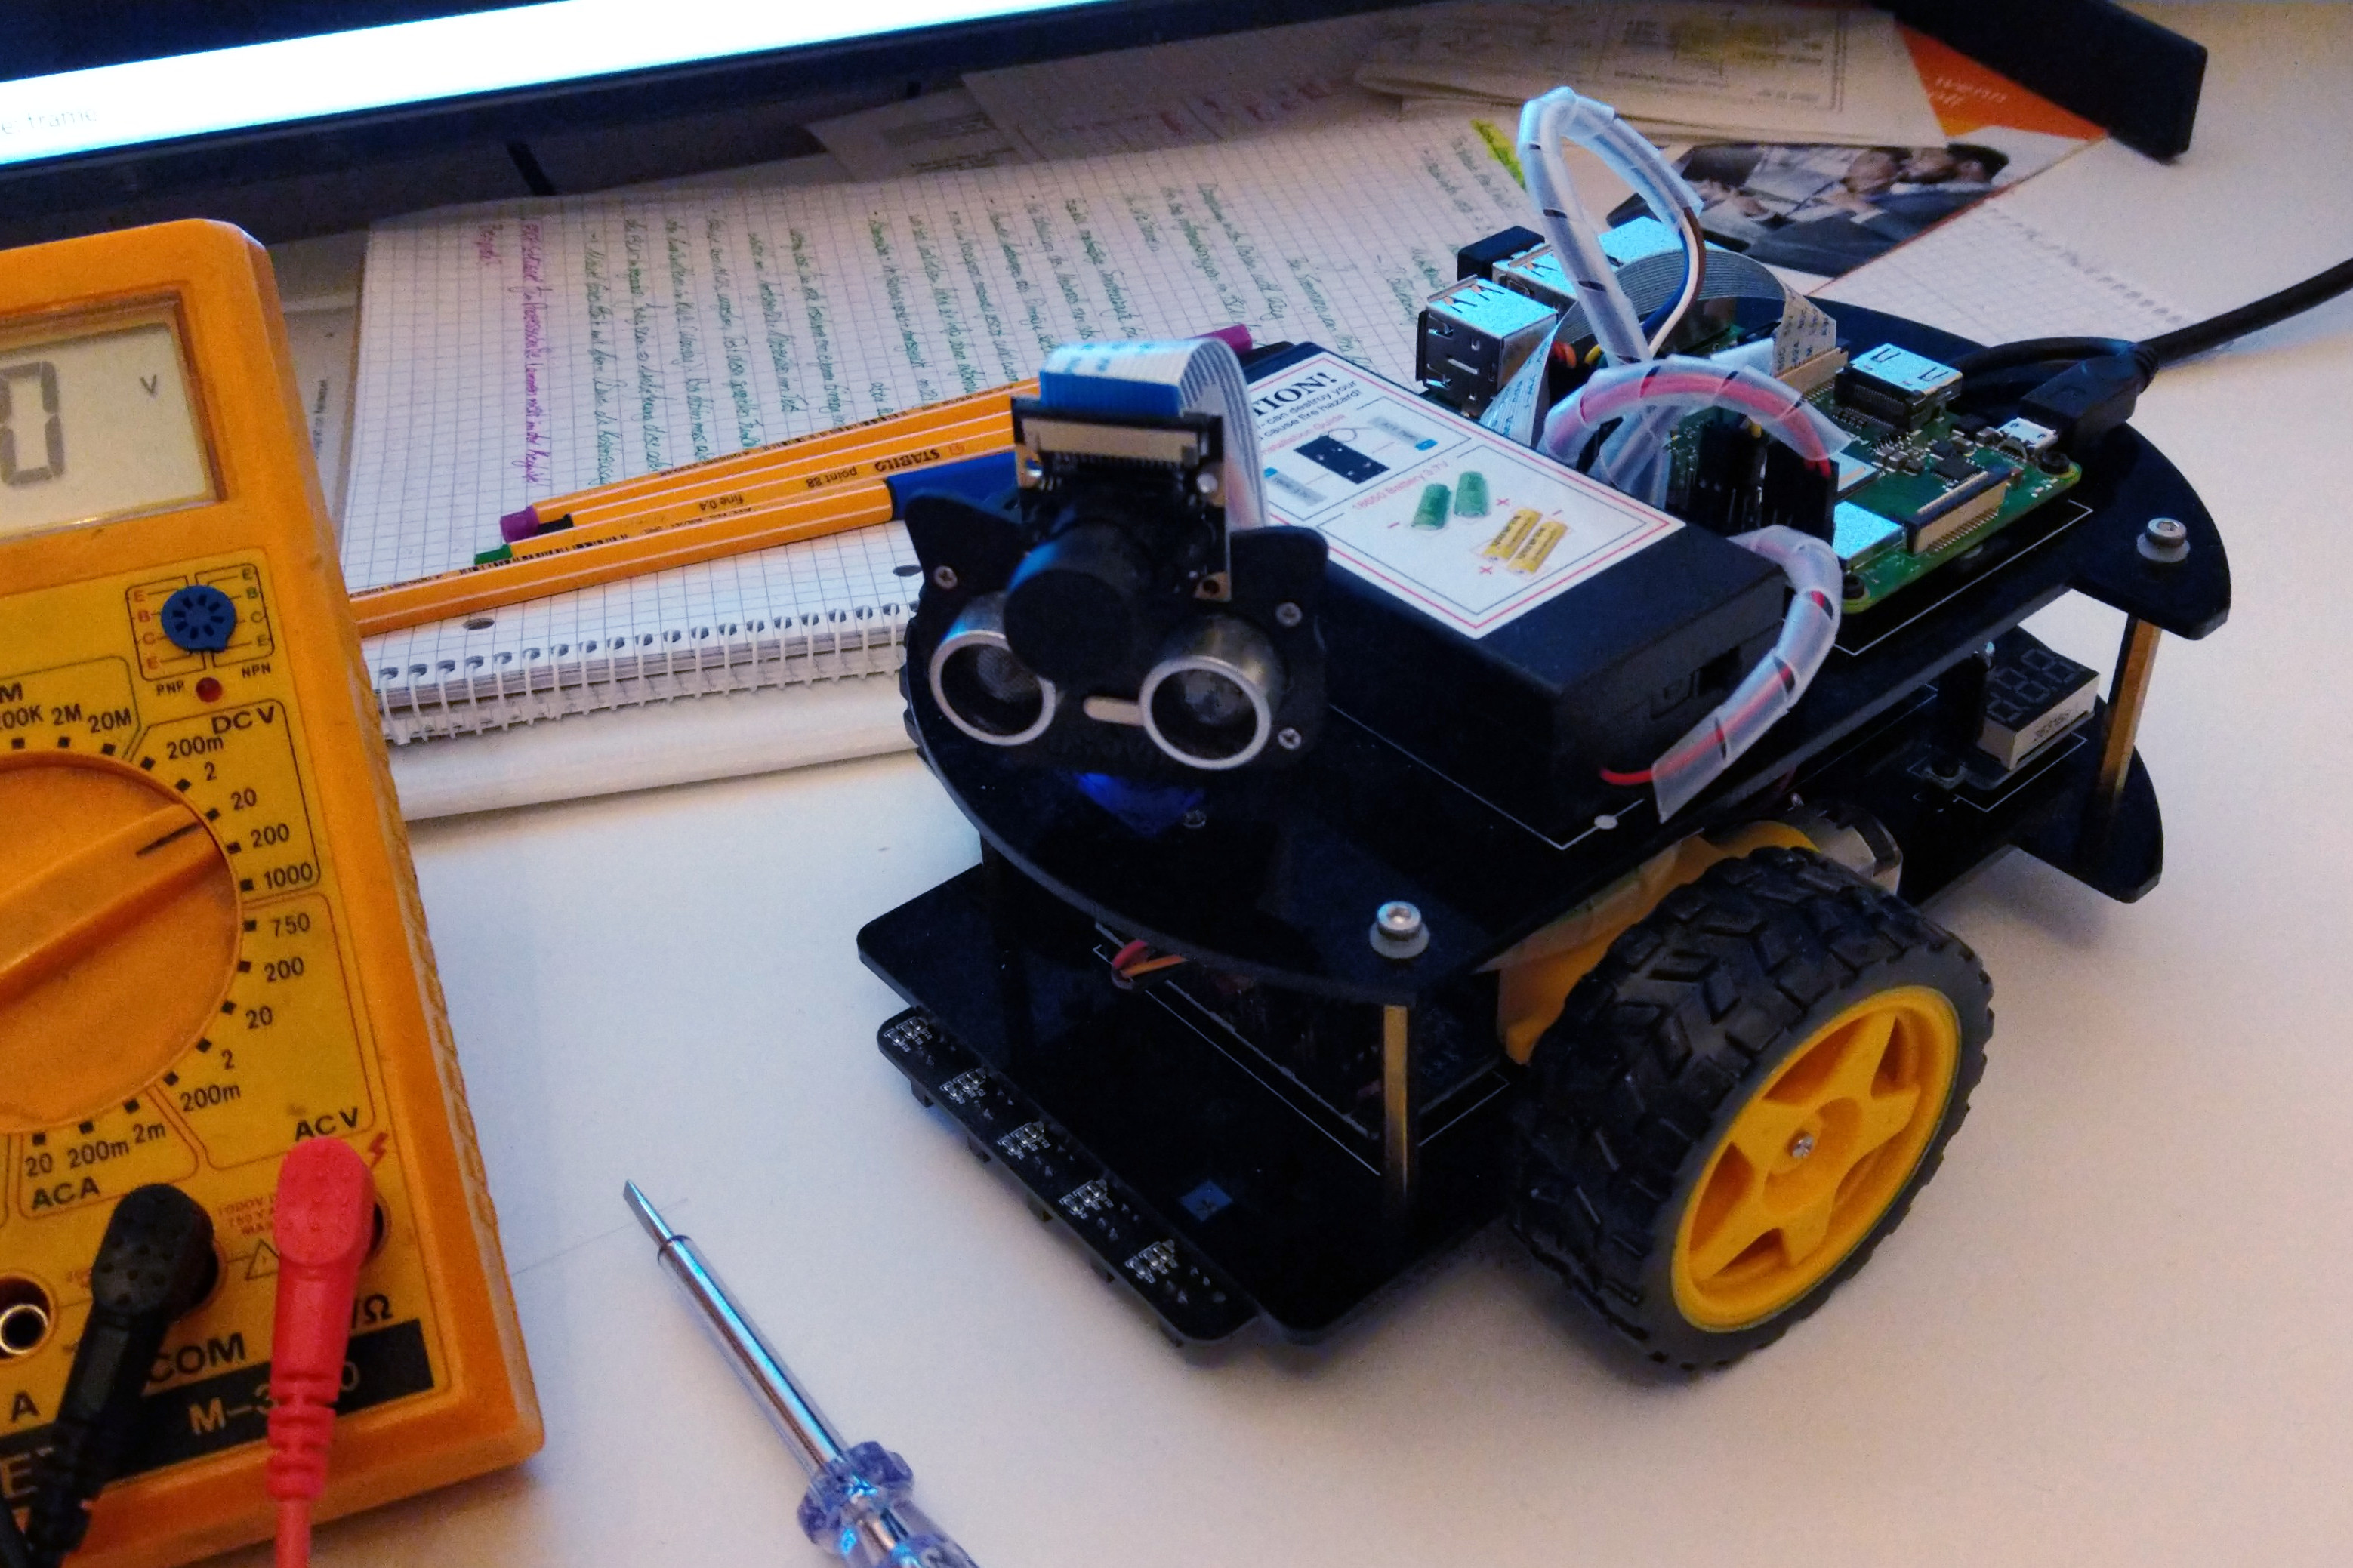
\includegraphics[height=\paperheight, width=\paperwidth]{img/fallbeispiel_fahrzeug}
    }

    \begin{frame}[plain]
    \end{frame}
}

%%% Folie
\begin{frame}{Häufig vorkommende Signalarten}
        \begin{columns}
        \column[b]{.5\textwidth}
        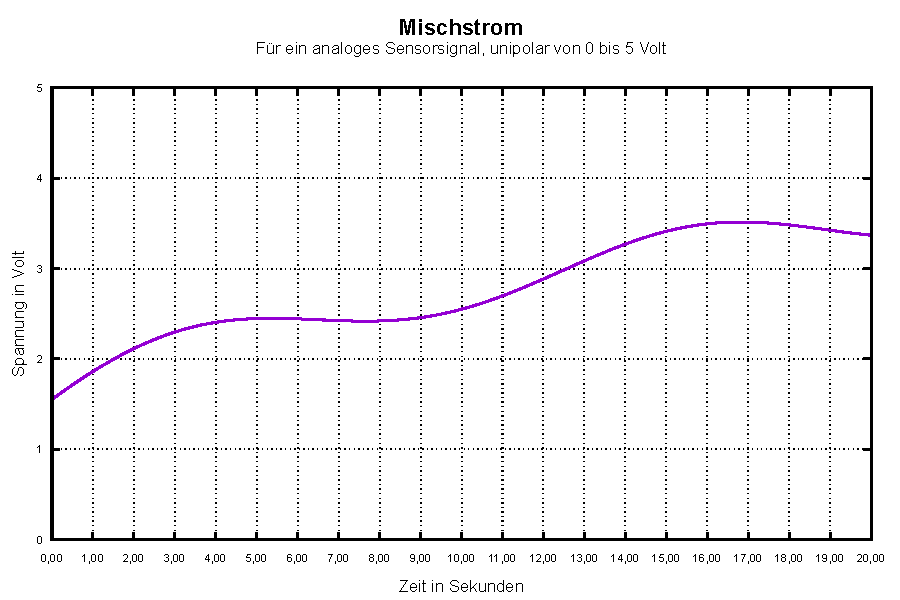
\includegraphics[width=\textwidth]{img/strom-analogsensor} \\

        \column[b]{.5\textwidth}
        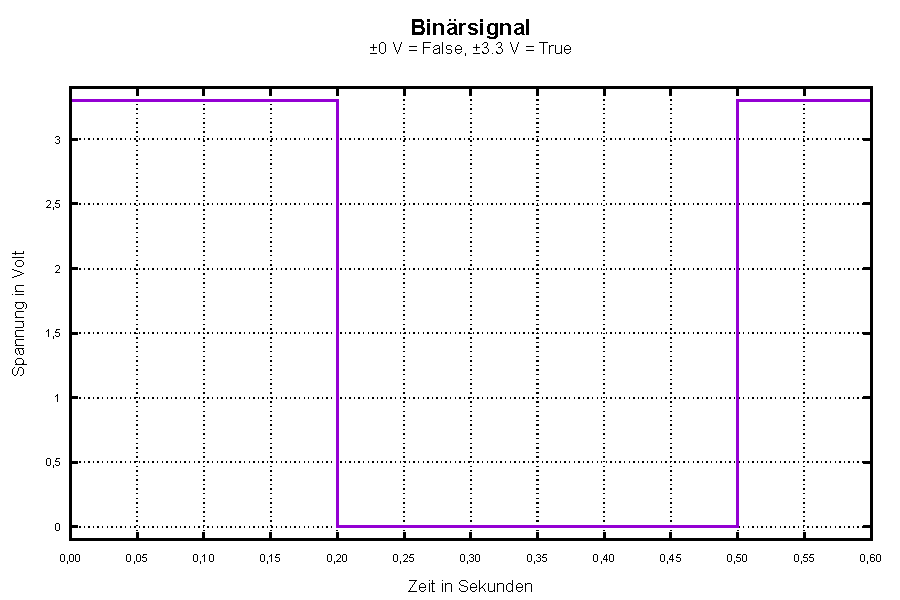
\includegraphics[width=\textwidth]{img/strom-binary} \\
    \end{columns}

    \bigskip

    \begin{columns}
        \column[b]{.5\textwidth}
        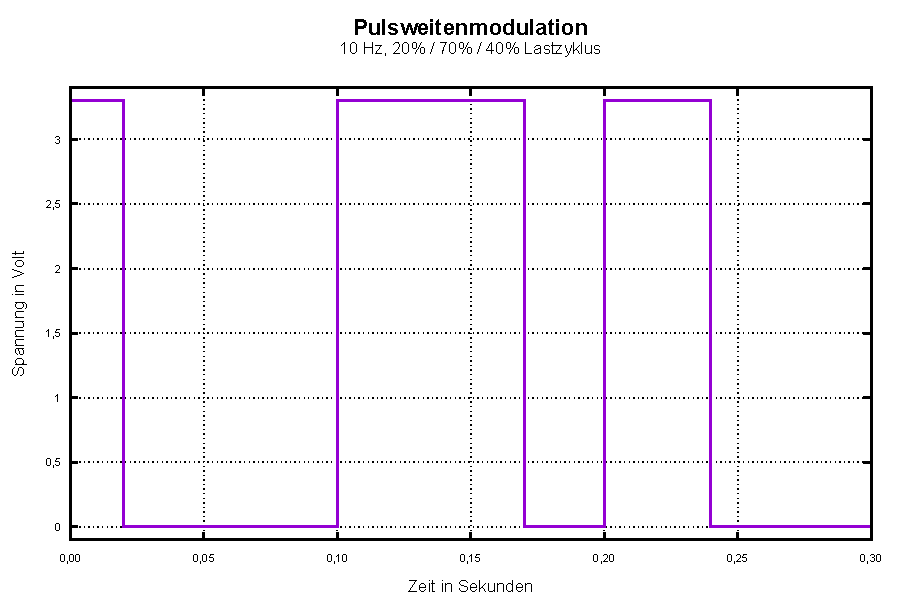
\includegraphics[width=\textwidth]{img/strom-pwm} \\

        \column[b]{.5\textwidth}
        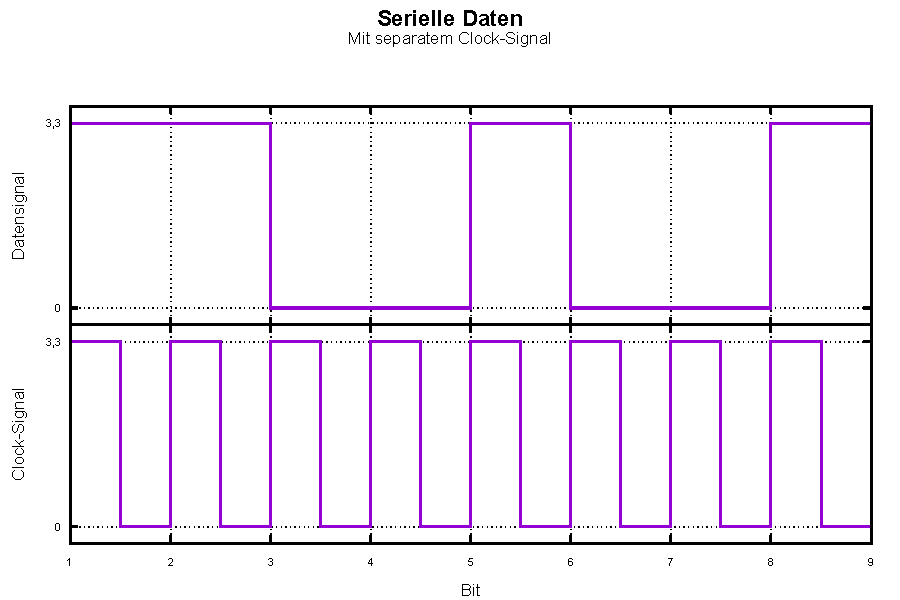
\includegraphics[width=\textwidth]{img/strom-serial} \\
    \end{columns}
\end{frame}

%%% Folie
\begin{frame}{Anschlüsse am Arduino Uno}
        \begin{center}
            \includegraphics[height=.8\textheight]{img/arduino-uno-pinout}

            \smallskip
            \LinkButton{https://docs.arduino.cc/hardware/uno-rev3}{Arduino Uno R3 Spezifikationen}
        \end{center}
\end{frame}

%%% Folie
\begin{frame}{Anschlüsse am Raspberry Pi}
        \begin{center}
            \includegraphics[height=0.5\textheight]{img/raspberry_anschluesse}
        \end{center}

        \smallskip

        \begin{columns}
            \begin{column}[T]{.5\textwidth}
                \begin{enumerate}
                    \item Mini-USB Stromversorgung
                    \item J8 GPIO-Header
                    \item Display Serial Interface
                    \item Camera Serial Interface
                \end{enumerate}
            \end{column}
            \begin{column}[T]{.5\textwidth}
                \begin{enumerate}
                    \setcounter{enumi}{4}   % Zielwert - 1
                    \item HDMI-Bildschirmanschluss
                    \item LAN-Netzwerkanschluss
                    \item USB (4 Stück)
                    \item WiFi, Bluetooth
                \end{enumerate}
            \end{column}
        \end{columns}
\end{frame}

%%% Folie
{
\footnotesize

\begin{frame}{Der J8 GPIO-Header im Detail}
        \begin{columns}
            \column[b]{.5\textwidth}
            \includegraphics[height=.7\textheight]{img/pinout}
            %\includegraphics[width=\textwidth]{img/raspberry_j8}

            \medskip
            \LinkButton{https://pinout.xyz/}{Raspberry Pi Pinout Guide}

            \column[b]{.5\textwidth}
            \begin{block}{Stromquellen}
                \begin{itemize}
                    \item 5V Power
                    \item 3.3V Power
                    \item Ground (Masse)
                \end{itemize}
            \end{block}

            \begin{block}{Digitale Ein-/Ausgänge}
                \begin{itemize}
                    \item GPIO
                    \item Pulsweitenmodulation
                    \item Asynchron serielle Kommunikation
                    \item Synchron serielle Kommunikation \\ (SPI, I²C, I²S, 1-Wire)
                \end{itemize}
            \end{block}

            \begin{alertblock}{Keine analogen Ein-/Ausgänge!}
            \end{alertblock}
        \end{columns}
\end{frame}
}

%%% Folie
{
\footnotesize

\begin{frame}{Bevor es losgehen kann: Maximale Grenzwerte}
    \parbox{\linewidth}{
        \scriptsize
        Um eine Beschädigung am Microcontroller-Board zu vermeiden, müssen folgende Grenzwerte
        unbedingt eingehalten werden. Ggf. müssen daher nach dem Ohmschen Gesetz berechnete
        Widerstände in Serie zu einem Bauteil angeschlossen werden, um die Stromstärke zu begrenzen.
        Ebenso muss die Summe aller zugeführten und entnommenen Ströme berechnet und ebenfalls
        begrenzt werden.
    }

    \bigskip
    \renewcommand{\arraystretch}{1.2}

    \begin{tabularx}{\textwidth}{|p{11em}|X|X|}
        \hline
        \textbf{Parameter}    &  \textbf{Arduino Uno}         &  \textbf{Rasbperry Pi}         \\  \hline
        Stromversorgung       &  6-20\,V, $\geq$ 250\,mA      &  5\,V, $\pm$ 3\,A (eher mehr)  \\  \hline
        Logikpegel            &  5\,V                         &  3,3\,V                        \\  \hline
        Stromentnahme 3.3\,V  &  Max. 50\,mA gesamt           &  Max. 50\,mA gesamt            \\  \hline
        Stromentnahme 5\,V    &  Max. 50\,mA gesamt           &  Max. 50\,mA gesamt            \\  \hline
        GPIO-Stromentnahme    &  Max. 20\,mA (40\,mA gesamt)  &  Max. 16\,mA (50\,mA gesamt)   \\  \hline
    \end{tabularx}

    \bigskip
    \includegraphics[width=.75\textwidth]{img/stromentnahme-raspi-schaltplan}

    \hfill%
    \CircuitJS{https://www.falstad.com/circuit/circuitjs.html?ctz=CQAgzCAMB0l3BWEBGGAmOaDsWyQBxoBsAnCViApJZdQgKYC0yyAUADIj7JEhr74QWIoP6DqyEADMAhgBsAzvXDQIkVmCzUSAFh18BIXfrBhek6uoDmQkeDO3BYBGihRWAJy48Dg477cqdQAjIRIkNAQkIh0KTX11AHcjPXteYScHdQAPEBiScHwKLDQTEmp9ZFcAJRkFAAdg+g8PAE8AHQUABQBLVlyiBApsVywdCGwkStcAcS6ASQB5RgBBAFcFKxkAOyt+vIReMB1JLCpwVOmQAFk6pU6AChmPAHs17YATAEp9waPICBYZAQPC8K7sF6JTrtACOnUgADVfocAiVRCRJFcABI9KwAC2hcIUYAANGAkblUJATJBXKgxuBIFMULN6ABbegKJTbej7KlHZAFekFMBoVxXADKABdXmyFFKACceADWvNCqEMx30JDQBWwBXUQA}
\end{frame}
}

%%% Folie
{
\tiny

\begin{frame}{Binärsignal ausgeben am Beispiel einer LED}
    \Justified{
        Jeder \textbf{GPIO-Pin} kann softwaregesteuert als \textbf{Eingang oder Ausgang} konfiguriert werden.
        Ausgangspins stellen eine Spannung von \textbf{ca. 3,3\,V} (Rasbperry Pi) bzw. \textbf{ca. 5\,V}
        (Arduino Uno) zur Verfügung, um eine logische Eins zu signalisieren, sowie \textbf{0\,V} (entspricht
        einer Verbindung gegen Masse) für eine logische Null.
        \smallskip

        Der entnommene Strom muss in der Regel durch einen \textbf{Widerstand} begrenzt werden.
        Da die verfügbare Spannung und die gewünschte Stromstärke bekannt sind, kann dieser mit
        dem \textbf{Ohmschen Gesetz} leicht berechnet werden. Dabei muss jedoch auch der innere
        Widerstand des angeschlossenen Bauteils, der nicht immer leicht zu ermitteln ist,
        berücksichtigt werden, da dieser den Gesamtwiderstand erhöht und die Strommenge dadurch
        zusätzlich begrenzt.
        \smallskip

        \textcolor{red}{
            \textbf{Raspberry Pi:} Die entnommenen Ströme dürfen nicht größer als 16\,mA und ihre Summe nicht größer als 50\,mA sein.
        }

        \textcolor{red}{
            \textbf{Arduino Uno}: Die entnommenen Ströme dürfen nicht größer als 20\,mA und ihre Summe nicht größer als 40\,mA sein.
        }
    }

    \bigskip

    \begin{columns}
        \column{0.5\textwidth}
        \includegraphics[width=\textwidth]{img/led_direkt_circuitjs}
        \smallskip

        \CircuitJS{https://www.falstad.com/circuit/circuitjs.html?ctz=CQAgjCAMB0l3BWcMBMcUHYMGZIA4UA2ATmIxAUgoqoQFMBaMMAKAHMRCUAWCsFTjwoo8UKCwBOnDAO7dRGQqLmiq2XCzBcQi5fJB5ss-QIAmdAGYBDAK4AbAC4M7dU+DFUYkVgBlpx0S5eFTEIazsAZzoQbGhscT9CGRi8XiCU3iowq0jo2PjISX8MnSUStQ1sDCpDAWxUkGJ+EohPFiqaoxAQpoD3NoB3Rub63l7u-UKh8Z7mhGbCrQFdEtqSs0tbR2dXfo9YVmm55vT5gULE5KMqdOvQkHComLjxKSS6tFLRO4qpr5jPmsfu1qgYundxndWuIjh8qJCGoUAEacBCEECYJDcDDECho8QAD26igoeFo81J8V4zQASlYIgAHJF0CQSACeAB0IgAFACWLCJlG+QgQxF4RnI1IEAHFuQBJADyDAAgjYImwrAA7NgCmiieZpSACeaS8ACACy9KiXIAFNKJAB7Gya0wASl1lHI9XRovi9VxUpAssVKrVGu1Hsgkopvu6CGCZqD8qVqvVWp1KLWmAExHqePIhSJqVoeCQTRLykT0roAFs6BEopq6LrDLjCJB0U025AA4mAMoOR01iIOAAnEgA1nRNSwgA}

        \column{0.5\textwidth}
        \includegraphics[width=\textwidth]{img/led_direkt_foto}
    \end{columns}
\end{frame}
}

%%% Folie
{
\tiny

\begin{frame}[fragile]{Binärsignale ausgeben mit Arduino}
    \begin{lstlisting}[language=C++, gobble=8]
        // Konstanten und globale Variablen
        const int MIN_PIN = 0;
        const int MAX_PIN = 19;
        bool output       = false;

        /**
         * Initialisierung der Hardware nach dem Einschalten
         */
        void setup() {
            // Alle GPIO-Pins als digitale Ausgänge konfigurieren
            for (int i = MIN_PIN; i <= MAX_PIN; i++) {
                pinMode(i, OUTPUT);
            }
        }

        /**
         * Unendlich oft ausgeführte Hauptprogrammlogik
         */
        void loop() {
            for (int i = MIN_PIN; i <= MAX_PIN; i++) {
                digitalWrite(i, output);
            }

            output = !output;
            delay(1000);
        }
    \end{lstlisting}
\end{frame}
}

%%% Folie
{
\tiny

\begin{frame}[fragile]{Binärsignale ausgeben mit Python auf dem Raspberry Pi}
    \begin{lstlisting}[language=Python, gobble=8]
        import RPi.GPIO as GPIO, time

        GPIO_LED = 21
        DELAY_S = 0.5

        if __name__ == "__main__":
            try:
                # GPIO-Pin initialisieren
                GPIO.setmode(GPIO.BCM)
                GPIO.setup(GPIO_LED, GPIO.OUT)

                # LED alle halbe Sekunde ein bzw. ausschalten
                led_status = False

                while True:
                    led_status = not led_status
                    GPIO.output(GPIO_LED, led_status)

                    print("LED ist an" if led_status else "LED ist aus")

                    time.sleep(DELAY_S)
            except KeyboardInterrupt:
                pass

            GPIO.cleanup()
    \end{lstlisting}

    \hfill
    \LinkButton{https://sourceforge.net/p/raspberry-gpio-python/wiki/Examples/}{Dokumentation zu RPi.GPIO}
\end{frame}
}

%%% Folie
{
\scriptsize

\begin{frame}{Exkurs: Stromstärke einer LED berechnen}
    \begin{columns}
        \begin{column}{.3\textwidth}
            \begin{center}
                {\tiny \textcolor{gray}{Stromstärke je Spannung}} \\
                \includegraphics[width=\textwidth]{img/kennlinie-diode}
                \bigskip

                \includegraphics[width=.7\textwidth]{img/komponenten_elementar_led}
            \end{center}
        \end{column}
        \begin{column}{.7\textwidth}
            \Justified{
                Leuchtdioden sind ein typisches Beispiel für \textbf{nicht-lineare Bauteile} auf Basis
                von \textbf{Halbleitern}, die nicht dem Ohmschen Gesetz folgen. Zwar gibt es auch hier
                einen Zusammenhang zwischen \textbf{Spannung, Stromstärke und Widerstand}. Dieser lässt
                sich aber nicht durch eine einfache lineare Funktion beschreiben. Typische LEDs besitzen
                stattdessen folgende Parameter, die in die Berechnung einfließen müssen:
            }

            \medskip
            \begin{center}
                \renewcommand{\arraystretch}{1.2}
                \begin{tabular}{|p{3em}|p{10em}|p{4em}|}
                    \hline
                    $I_F$ & Maximale Stromstärke & 20\,mA \\
                    \hline
                    $V_D$ & Vorwärtsspannung & $\varnothing$ 2,2\,V \\
                    \hline
                \end{tabular}
            \end{center}
            \medskip

            \Justified{
                Die Lichtintensität hängt direkt von der Stromstärke ab, wobei diese in der Regel
                20\,mA nicht übersteigen darf. Um \textbf{näherungsweise} mit dem Ohmschen Gesetz
                den \textbf{Vorwiderstand} berechnen zu können, muss die \textbf{Vorwärtsspannung}
                (auch \textbf{Spannungsabfall} oder auf englisch Voltage Drop genannt) abgezogen
                werden. Der gesuchte Widerstand muss daher mit 1,1\,V anstatt 3,3\,V berechnet
                und anschließend auf den nächsten, tatsächlich als Bauteil verfügbaren Wert
                aufgerundet werden.
            }

            \begin{block}{Beispiel}
                \smallskip
                Die Stromstärke soll auf etwa 5\,mA begrenzt werden:
                \smallskip

                $R = \frac{3,3\,V - 2,2\,V}{0,005\,A} = \frac{1,1\,V}{0,005\,A} = 220\,\Omega$
                \smallskip

                \textcolor{red}{
                    Die tatsächliche Stromstärke wird geringfügig vom Sollwert abweichen.
                    In der Elektronik gilt daher immer: Konservativ rechnen und viel Puffer vorsehen.
                }
            \end{block}
        \end{column}
    \end{columns}
\end{frame}
}

%%% Folie
{
\scriptsize

\begin{frame}{Exkurs: Mittlere Lasten über Transistor schalten}
    \Justified{
        Der vom Raspberry Pi abgegebene Strom ist in der Regel zu schwach, um damit mehr
        als digitale Sensoren oder Aktoren anzusteuern. Insbesondere mechanische Arbeiten
        können damit nicht verrichtet werden, da die jeweiligen Motoren deutlich mehr Strom
        benötigen. Bei mittleren Lastströmen kann ein Transistor hier Abhilfe schaffen.
        \smallskip

        Der hier gezeigte ,,NPN-Transistor'' funktioniert im einfachsten Fall wie ein
        \textbf{stromgesteuerter Schalter}. \textcolor{RoyalPurple}{Ein kleiner Strom
        an der Basis steuert, in wiefern ein viel größerer am Collector anliegender Strom
        durchgelassen wird. Die Summe beider Ströme (in Ampére) fließt durch den Emitter
        nach Ground.}
        \smallskip

        Die Spannung zwischen Basis und Emitter muss meist mindestens 0,7V betragen,
        damit der Transistor schalten kann. Die Stärke des hierfür benötigten
        Steuer- bzw. Basisstroms kann mit der durchzuschaltenden Stromstärke, dem
        $\beta$-Faktor des Transistors, (auch \texttt{hfe} abgekürzt) und dem Ohmschen
        Gesetz leicht berechnet werden:
        \bigskip

        \hfill $I_b = I_c / \beta$ \hfill
        \hfill \textit{Benötigter Basisstrom = Zu schaltender Strom / $\beta$} \hfill
        \smallskip
    }

    \bigskip

    \begin{columns}[T]
        \column{0.5\textwidth}
        \includegraphics[width=\textwidth]{img/led_transistor_circuitjs}
        \smallskip

        \CircuitJS{https://www.falstad.com/circuit/circuitjs.html?ctz=CQAgjCAMB0l3BWcMBMcUHYMGZIA4UA2ATmIxAUgoqoQFMBaMMAKABkRiAWLkLsQiDxc8fAVHAgAZgEMANgGc6IbNGxQWAcyEi+xQcNEIwKCZBYB3cCapd9O0XcHmASpx4rsB3di9m+tP4wCCwATu68-IJgkAiCURIxcCwALshxYtE2mYlQ0IRgxGCU3Hh4xJAouLwwhIR2cAII2GQIzbxJIAAmdLIArnIpltZofNimzKNOGuHcvL7RsYILEr7mVjEZK5NUK+YARkJ4u5C8GKcUXOrmAB4g56ZtxPdYFISmHaYuMgoADvt0UKhACeAB0FAAFACWLDuGBQpmw-HuCFESMi4FMEIA9hZAbD7lNRsd4lU+JiQABxCEASQA8gwAIJ9BSaGQAO00BIwhRoVDwYHUlHUnxAAFkfkpwQAKSmhbF9dldACULAEE2y22yXDgIFMPX6gwYcjoXUkVAtsFYdxidQCohiZDEEFFACEflCFATJs8dVRmAQAiKKQBhbFyE0AYxS2NC3pMvt81hwY3iFIAogBbKEpFL4oA}
        \LinkButton{https://www.electronics-tutorials.ws/de/transistoren/der-npn-transistoren.html}{NPN-Transistoren im Detail}

        \column{0.42\textwidth}
        \includegraphics[width=\textwidth]{img/led_transistor_foto}
    \end{columns}
\end{frame}
}

%%% Folie
{
\scriptsize

\begin{frame}{Exkurs: Große Lasten über Relais schalten}
    \Justified{
        Große Lasten können aus Sicherheitsgründen nur mechanisch geschaltet werden.
        Der Hardwareaufbau gliedert sich dann ein einen \textbf{Steuerstromkreis} und
        einen \textbf{Arbeitsstromkreis}, die komplett \textbf{galvanisch entkoppelt}
        sind und deshalb jeweils eigene Stromquellen besitzen.
        Ein \textbf{Relais} dient als ferngesteuerter Schalter, der den Arbeitsstromkreis
        unterbrechen und schließen kann. Im Inneren besteht es aus einem durch den
        Steuerstromkreis gespeisten Elektromagneten und einem magnetischen Kippschalter.
        Beim Umschalten entsteht das charakteristische Klickgeräusch.
    }

    \medskip

    \begin{columns}
        \column{0.6\textwidth}
        \includegraphics[width=.9\textwidth]{img/led_relais_circuitjs}
        \smallskip

        \CircuitJS{https://www.falstad.com/circuit/circuitjs.html?ctz=CQAgjCAMB0l3BWcMBMcUHYMGZIA4UA2ATmIxAUgoqoQFMBaMMAKABkQ9jCQAWMHnl54+AqOBAAzAIYAbAM50Q2aNigsA5p2F9u2kQjApxkFgCdOe-jzI9r4zKYBGnPFWxCQGSLwq81pgAeXpDGCAjEXlgUhMa+RiAAStLyAA5OdGZmAJ4AOvIACgCWLMEYaHwVbnYoavHGAOIFAJIA8gwAggCu8hrSAHYapV5gkZRUeGBqlHXgxgCyKYr5ABQNZgD2Xf0AJgCULGAYIrbKnmD4Ih6+PBCoULDM2BjE2BfYvMKYvITkMJBIC7wOAPSAQCr-HyggHgFgAd3ARio9mYFV4elMCNRyL0QhE6J4QWQFUMtyMYVGfDmIAAygAXOhdTLyOmbAC2AGszHQivJDpNLDwUAhbqFfMLCeBiCheLAhIZuJQpngeJRqf9fBr4YiKhKdciQZjkHh8SDsXxDdrzSjLqJCcMLmARDK1Ki1DK7NSOmYMkU6fIWeyuTy+Vo8cooeHsBD1Aio1DTrhNdrEwmMDxrupEoKQHrw3qqAb1SZoAgrWLcyL9ZX7S4TVQ0CJvGoPsmypBXcQRHgEOQ0BB6iAAKKBBlmfp0fL09kAN2ZGzMGm2QyAA}

        \column{0.4\textwidth}
        \includegraphics[width=\textwidth]{img/led_relais_foto}
    \end{columns}
\end{frame}
}

%%% Folie
{
\scriptsize

\begin{frame}{Gemittelte Leistung durch Pulsweitenmodulation regulieren}
    \parbox{\linewidth}{
        Die zur Verfügung stehende Stromstärke kann nicht nur durch einen Vorwiderstand reduziert werden.
        Je nach Bauteil kann (oder muss) sie durch \textbf{Pulsweitenmodulation}, was einem schnellen
        Ein- und Ausschalten entspricht, im zeitlichen Mittel reduziert werden. Die zwei wesentlichen
        Parameter sind die \textbf{Frequenz} und der \textbf{Tastgrad} (Duty Cycle):
    }

    \begin{center}
        \includegraphics[width=.8\textwidth]{img/pwm} \\
        \bigskip

        \includegraphics[width=.75\textwidth]{img/led_pwm_circuitjs}
    \end{center}

    \hfill
    \CircuitJS{https://www.falstad.com/circuit/circuitjs.html?ctz=CQAgjCAMB0l3BWcMBMcUHYMGZIA4UA2ATmIxAUgoqoQFMBaMMAKAHMRCUAWCsFTjwoo8UKCwBOnDAO7dRGQqLmiq2XCzBcQi5fJB5ss-QIAmdAGYBDAK4AbAC4M7dU+DFUYkVgBlpA7DxeLl5A3ioIazsAZzoQbGhscSlCGXignSV08PiNbAwqQwCM4n5s908WfMKjEBUQUuNRCEqAdwaysI6m8XbGuv1+hDLIFj6y4YEQvgFRgCNOBEJc4jqMVYQl8QAPNeWEPFphikM68AEAJStogAc5ugkJAE8AHWiABQBLFl3KDa1OJAksNVrwygBZa6xN4ACgA4hIAPY2AB2pgAlD8aORAvtiElAqDziA4e8AJIAeQYAEEbNE2FYUWwsZRyNxjghiLIELwwQJ3gB1cE0ukMpksBZFXLLMD4ASbcijXZBWh4JClVXKYlwugAWzo0ViKLoWMMq0IkGWpXNkCJZQAyg4kbrog4ACcSADWdBRmm0unKUq6ZkstkczlcFQ8sFYF38A1E03qvCQsrUiQ8UES2BY3CBDREdVqsrS8k8nAA+kYK5AK1p1uya7B4IoUPjiOzsPwEE24Fwe7WUBXCFWWEA}
\end{frame}
}

%%% Folie
{
\scriptsize

\begin{frame}[fragile]{Pulsweitenmodulation mit Arduino}
    \begin{lstlisting}[language=C++, gobble=8]
        // Konstanten und globale Variablen
        const int PIN_OUTPUT = 13;

        /**
         * Initialisierung der Hardware nach dem Einschalten
         */
        void setup() {
            pinMode(PIN_SIN, OUTPUT);
        }

        /**
         * Unendlich oft ausgeführte Hauptprogrammlogik
         */
        void loop() {
            for (int pulse_width = 0; pulse_width < 255; pulse_width++) {
                analogWrite(PIN_OUTPUT, pulse_width);
                delay(100);
            }
        }
    \end{lstlisting}

    \bigskip

    \Justified{
        \texttt{analogWrite()} erzeugt auf den meisten Arduino-Boards ein PWM-Signal
        mit fester Frequenz um diee 500\,Hz. Lediglich der Tastgrad kann als 8-Bit
        Integer verändert werden. Für eine genauere Steuerung müsste das PWM-Signal
        entweder per Bit-Banging manuell generiert oder eine Library verwendet werden.
    }
\end{frame}
}

%%% Folie
{
\tiny

\begin{frame}[fragile]{Pulsweitenmodulation ausgeben mit Raspberry Pi}
    \begin{lstlisting}[language=Python, gobble=8]
        import RPi.GPIO as GPIO, time

        GPIO_LED   = 12
        FREQUENCY  = 100    # 100 Hz
        DUTY_CYCLE = 50     # 50%

        if __name__ == "__main__":
            try:
                # GPIO-Pin initialisieren
                GPIO.setmode(GPIO.BCM)
                GPIO.setup(GPIO_LED, GPIO.OUT)

                # Pulsweitenmodulation einstellen
                led_pwm = GPIO.PWM(GPIO_LED, FREQUENCY)
                led_pwm.start(DUTY_CYCLE)

                # Endlosschleife, damit das Programm nicht beendet wird
                while True:
                    time.sleep(10)

            except KeyboardInterrupt:
                pass

            GPIO.cleanup()
    \end{lstlisting}
\end{frame}
}

%%% Folie
{
\small
\setlength{\leftmargini}{1.2em}

\begin{frame}{Pulsweitenmodulation am Beispiel eines Servomotors}
    \begin{columns}[onlytextwidth]
        \column{.49\textwidth}
        \includegraphics[width=\textwidth]{img/servomotor-foto1}

        \column{.49\textwidth}
        \includegraphics[width=\textwidth]{img/servomotor-foto2}
    \end{columns}

    \bigskip
    Steuerung eines Servomotors mit Pulsweitenmodulation. Die Länge des Lastzyklus
    bestimmt die Position:

    {
        \footnotesize
        \smallskip
        \begin{itemize}
            \item \textbf{Ganz links:} 1\,ms Puls bei 50\,Hz Frequenz
            \item \textbf{Ganz rechts:} 2\,ms Puls bei 50\,Hz Frequenz
            \item \textbf{Andere:} Jeder Wert dazwischen
        \end{itemize}
    }

    \begin{columns}[onlytextwidth]
        \column[T]{.3\textwidth}
        \begin{block}{Hardwareskizze}
            \smallskip
            \includegraphics[width=\textwidth]{img/servomotor-skizze}
        \end{block}

        \column[T]{.59\textwidth}
        \begin{block}{Schaltplan}
            \smallskip
            \includegraphics[width=\textwidth]{img/servomotor-schaltplan}
        \end{block}
    \end{columns}
\end{frame}
}

%%% Folie
{
\scriptsize

\begin{frame}{Digitaleingang mit Active-High-Logik (z.B. Taster)}
    \Justified{
        Viele Sensoren stellen lediglich einen \textbf{Kontakt zwischen zwei Pins} her, wenn ein bestimmtes
        Ereignis eintritt, zum Beispiel wenn ein Schalter gedrückt, eine Berührung mit einem Hindernis
        oder ein Feuer erkannt wird. Indem man einen Pin des Sensors mit einer 3,3\,V Versorgungsspannung
        und den anderen Pin mit einem GPIO-Eingang verbindet, lässt sich eine sog. \textbf{Active-High-Logik}
        realisieren. Dies bedeutet, dass der GPIO-Eingang durch den Sensor mit 3,3\,V gespeist wird,
        wenn das Ereignis eintritt, was vom Raspberry Pi als logische Eins interpretiert wird.
        \smallskip

        Jedoch sollte in diesem Fall immer der \textbf{interne Pull-Down-Widerstand} des Raspberry Pi
        aktiviert werden, um den Eingang auf Masse zu ziehen, wenn kein Signal anliegt. Andernfalls
        führen \textbf{parasitäre Induktionen} zu zufälligen Phantomwerten und Fehlmessungen.
        \medskip
    }

    \begin{columns}
        \column{0.6\textwidth}
        \includegraphics[width=\textwidth]{img/button_pulldown_circuitjs}
        \bigskip

        \CircuitJS{https://www.falstad.com/circuit/circuitjs.html?ctz=CQAgjCAMB0l3BWcMBMcUHYMGZIA4UA2ATmIxAUgoqoQFMBaMMAKAFkQ9sUQAWPKjkJ8BUECmgIWADxCEUPXhl4gMkFUvIqwPAOIAFAJIB5BgFEAlgDsA5gENbLAM4hiOkVVKLRVCADM7ABsnOhYAJU5uPjhVbGFeGKoqBJBsaGwxJMkWG1jhBEJBOIoMYSSWAHc8ikLVPBUC8oAnOo1RDHqapJp4GTkFPmIVEmSyPnAeAEEAYwAXCwA3OgAdJwAJCxsACz75HgKMjDB8wniJkDY7JxDVgApdJoB7AFcrABMASkrXYm9PX+i5SqXkBkUUiRYLS4f1c7n43TAvVkeE68gyiLASHkZ3c+megUCDAAIo8KlYGAB1CxvOhNJyzBxvPpucgIDDEZB4DkIAjjdwAIToNiadCsAC9XjZVjSmqsAMqzJ4AW3pABOmgBrUKyNzcwgQDG0Qgac5UmX0xmrCVNFi8FAZYjFBC8FQoxRDKC2+2cYhUQpIAR4CjYFSQFgAIzBqUIQcKsfwntk8iDCQgpw06j5PH0pNpu2Y-WGeGE8i05zCVwADuHaU0AJ6rfQWFhAA}

        \column{0.4\textwidth}
        \includegraphics[width=\textwidth]{img/button_pulldown_foto}
    \end{columns}
\end{frame}
}

%%% Folie
{
\scriptsize

\begin{frame}[fragile]{Active-High-Eingang mit Arduino}
    \begin{lstlisting}[language=C++, gobble=8]
        // Konstanten und globale Variablen
        const int PIN_BUTTON = 2;
        const int PIN_LED = 13;

        /**
         * Initialisierung der Hardware nach dem Einschalten
         */
        void setup() {
            pinMode(PIN_BUTTON, INPUT);
            pinMode(PIN_LED, OUTPUT);
        }

        /**
         * Unendlich oft ausgeführte Hauptprogrammlogik
         */
        void loop() {
            bool button_pressed = digitalRead(PIN_BUTTON);
            digitalWrite(PIN_LED, button_pressed);
        }
    \end{lstlisting}

    \bigskip

    \Justified{
        Digital Eingänge, die in mit \texttt{pinMode()} als \texttt{INPUT} deklariert
        werden, werden immer mit Active-High-Logik abgefragt. Eingänge, die als
        \texttt{INPUT\_PULLUP} konfiguriert werden mit Active-Low-Logik, da der
        interne Pull-Up-Widerstand den Eingang dauerhaft auf 5\,V hochzieht und
        dieser durch den angeschlossenen Sensor nur nach gegen Masse kurzgeschlossen
        werden kann, um eine Änderung zu signalisieren.
        \smallskip

        Darüber hinaus muss auf dem Arduino nichts beachtet werden. Bis auf die
        Konstante bei \texttt{pinMode()} erfordert die Programmierung keinerlei
        Sonderlogik zur Unterscheidung von Active-High- und Active-Low-Komponenten.
    }
\end{frame}
}

%%% Folie
{
\scriptsize

\begin{frame}[fragile]{Active-High-Eingang mit Raspberry Pi}
    \begin{lstlisting}[language=Python, gobble=8]
        import RPi.GPIO as GPIO, time

        GPIO_BUTTON = 22

        def on_button_event(button):
            """Button-Callback. Läuft in einem eigenen Thread!"""

            if GPIO.input(button) == GPIO.HIGH:
                print("Der Button WIRD GEDRÜCKT")
            else:
                print("Der Button WURDE LOSGELASSEN")

        if __name__ == "__main__":
            try:
                # GPIO-Pins initialisieren
                GPIO.setmode(GPIO.BCM)
                GPIO.setup(GPIO_BUTTON, GPIO.IN, pull_up_down=GPIO.PUD_DOWN)

                GPIO.add_event_detect(GPIO_BUTTON, GPIO.BOTH)   # GPIO.RISING, GPIO.FALLING
                GPIO.add_event_callback(GPIO_BUTTON, on_button_event)

                # Endlosschleife, damit das Hauptprogramm weiterläuft
                while True:
                    time.sleep(10)
            except KeyboardInterrupt:
                pass

            GPIO.cleanup()
    \end{lstlisting}
\end{frame}
}

%%% Folie
{
\scriptsize

\begin{frame}{Digitaleingang mit Active-Low-Logik (z.B. Lichtschranke)}
    \Justified{
        Einige Sensoren \textbf{unterbrechen einen Kontakt}, wenn die festzustellende Bedingung eintritt.
        Dies trifft zum Beispiel auf Lichtschranken zu, die an ihrem Ausgang so lange einen Strom liefern,
        bis sie unterbrochen werden. Am einfachsten lassen sich solche Sensoren wie hier gezeigt mit einer
        \textbf{Active-Low-Logik} verbinden.
        Indem der interne Pull-Up-Widerstand des Raspberry Pi aktiviert wird, wird der GPIO-Eingang bei
        einer Unterbrechung des Eingangssignals auf eine logische Eins hochgezogen. Die meiste Zeit kann
        der Strom jedoch über den Sensor nach Masse abfließen, so dass der Raspberry Pi stattdessen eine
        logische Null sieht.
    }

    \bigskip

    \begin{columns}
        \column{0.6\textwidth}
        \includegraphics[width=\textwidth]{img/button_pullup_circuitjs}
        \bigskip

        \CircuitJS{https://www.falstad.com/circuit/circuitjs.html?ctz=CQAgjCAMB0l3BWcMBMcUHYMGZIA4UA2ATmIxAUgoqoQFMBaMMAKAFkQM8AWEbvKjkJ8BUECmgIWADxCEUKPhl4ZIvblj7hFAcQAKASQDyDAKIBLAHYBzAIY2WAZxDEwi-lVLvRVCADNbABtHOhYAJU4ePjhObGFuGKoqBJBsaGwxJMkWa1jhBEJBOIoMYSSWAHc8ikLI3gLygCc66MEojzFKeBk5BT5iXkI8eLItNxAAQQBjABdzADc6AB1HABkAewqe+UUCjIwwfMJ47RA2W0cQlYAKHUb1gFdLABMASkqXYl3arnrayB6wwy2GISDI5BBeDGij0D0CgQYAFUAA4MADq5medEajhm9meLG4KAyw2I0QgeDAZO4RKgLAARiA8NhFHEoYV2fg6bJ5FCEhBjuo1NCQHpNtjtsxeoNhr1yLxxmELsj6djGgBPFZ6cwfVzeNrqHwsZpeESeL41JKpXA9Yh4JCEXDIUpybAZBWKDFYnF4l4rABeD0atqihG4ZOYBTkCHcpwAQnRrI06JZAzYVt6VgBlGb3AC2uIAJ40ANahIkZMCQFBkwhgJBVsDkBApAFAA}

        \column{0.4\textwidth}
        \includegraphics[width=\textwidth]{img/button_pullup_foto}
    \end{columns}
\end{frame}
}

%%% Folie
{
\scriptsize

\begin{frame}[fragile]{Active-Low-Eingang mit Arduino}
    \begin{lstlisting}[language=C++, gobble=8]
        // Konstanten und globale Variablen
        const int PIN_BUTTON = 2;
        const int PIN_LED = 13;

        /**
         * Initialisierung der Hardware nach dem Einschalten
         */
        void setup() {
            pinMode(PIN_BUTTON, INPUT_PULLUP);      // Einzige Änderung zu davor
            pinMode(PIN_LED, OUTPUT);
        }

        /**
         * Unendlich oft ausgeführte Hauptprogrammlogik
         */
        void loop() {
            bool button_pressed = digitalRead(PIN_BUTTON);
            digitalWrite(PIN_LED, button_pressed);
        }
    \end{lstlisting}

    \bigskip

    \Justified{
        Digital Eingänge, die in mit \texttt{pinMode()} als \texttt{INPUT} deklariert
        werden, werden immer mit Active-High-Logik abgefragt. Eingänge, die als
        \texttt{INPUT\_PULLUP} konfiguriert werden mit Active-Low-Logik, da der
        interne Pull-Up-Widerstand den Eingang dauerhaft auf 5\,V hochzieht und
        dieser durch den angeschlossenen Sensor nur nach gegen Masse kurzgeschlossen
        werden kann, um eine Änderung zu signalisieren.
        \smallskip

        Darüber hinaus muss auf dem Arduino nichts beachtet werden. Bis auf die
        Konstante bei \texttt{pinMode()} erfordert die Programmierung keinerlei
        Sonderlogik zur Unterscheidung von Active-High- und Active-Low-Komponenten.
    }
\end{frame}
}

%%% Folie
{
\scriptsize

\begin{frame}[fragile]{Active-Low-Eingang mit Raspberry Pi}
    \begin{lstlisting}[language=Python, gobble=8]
        import RPi.GPIO as GPIO, time

        GPIO_BUTTON = 22

        def on_button_event(button):
            """Button-Callback. Läuft in einem eigenen Thread!"""

            if GPIO.input(button) == GPIO.HIGH:
                print("Die Lichtschranke WURDE UNTERBROCHEN")
            else:
                print("Die Lichtschranke WIRD NICHT MEHR UNTERBROCHEN")

        if __name__ == "__main__":
            try:
                # GPIO-Pins initialisieren
                GPIO.setmode(GPIO.BCM)
                GPIO.setup(GPIO_BUTTON, GPIO.IN, pull_up_down=GPIO.PUD_UP)   # <-- Hier!

                GPIO.add_event_detect(GPIO_BUTTON, GPIO.BOTH)
                GPIO.add_event_callback(GPIO_BUTTON, on_button_event)

                # Endlosschleife, damit das Hauptprogramm weiterläuft
                while True:
                    time.sleep(10)
            except KeyboardInterrupt:
                pass

            GPIO.cleanup()
    \end{lstlisting}
\end{frame}
}

%%% Folie
%{
%\setlength{\leftmargini}{1.2em}
%\footnotesize

%\begin{frame}[fragile,allowframebreaks]{Zusammenfassung zur Programmierung in Python}
    %\begin{block}{Initialisieren und Zurücksetzen der GPIO-Pins}
        %\begin{lstlisting}[style=MethodenListe, gobble=12]
            %import RPi.GPIO as GPIO
        %\end{lstlisting}
        %Raspberry Pi GPIO-Modul importieren
        %\medskip

        %\begin{lstlisting}[style=MethodenListe, gobble=12]
            %GPIO.setup(10, GPIO.OUT)
        %\end{lstlisting}
        %GPIO\,10 als Ausgang konfigurieren
        %\medskip

        %\begin{lstlisting}[style=MethodenListe, gobble=12]
            %GPIO.setup(11, GPIO.IN)
        %\end{lstlisting}
        %GPIO\,11 als Eingang konfigurieren
        %\medskip

        %\begin{lstlisting}[style=MethodenListe, gobble=12]
            %GPIO.setup(12, GPIO.IN, pull_up_down=GPIO.PUD_DOWN)
        %\end{lstlisting}
        %GPIO\,12 als Eingang mit internem Pull Down konfigurieren
        %\medskip

        %\begin{lstlisting}[style=MethodenListe, gobble=12]
            %GPIO.setup(13, GPIO.IN, pull_up_down=GPIO.PUD_UP)
        %\end{lstlisting}
        %GPIO\,13 als Eingang mit internem Pull Up konfigurieren
        %\medskip

        %\begin{lstlisting}[style=MethodenListe, gobble=12]
            %GPIO.cleanup()
        %\end{lstlisting}
        %Alle GPIO-Pins auf eine sichere Standardkonfiguration zurücksetzen
        %\medskip
    %\end{block}

    %\framebreak

    %\begin{block}{Lesen und Schreiben einzelner Pins}
        %\begin{lstlisting}[style=MethodenListe, gobble=12]
            %value = GPIO.input(14)
        %\end{lstlisting}
        %Aktuellen Zustands von GPIO\,14 (True oder False) lesen
        %\medskip

        %\begin{lstlisting}[style=MethodenListe, gobble=12]
            %GPIO.output(15, True)
        %\end{lstlisting}
        %GPIO\,15 auf High bzw. 3,3\,V Spannung setzen
        %\medskip

        %\begin{lstlisting}[style=MethodenListe, gobble=12]
            %GPIO.output(16, False)
        %\end{lstlisting}
        %GPIO\,16 auf Low bzw. 0\,V Spannung setzen
        %\medskip
    %\end{block}

    %\begin{block}{Reagieren auf Interrupts}
        %\begin{lstlisting}[style=MethodenListe, gobble=12]
            %GPIO.add_event_detect(17, GPIO.RISING, mein_cb)
        %\end{lstlisting}
        %Callback-Funktion für steigende Flanken auf GPIO\,17 registrieren
        %\medskip

        %\begin{lstlisting}[style=MethodenListe, gobble=12]
            %GPIO.add_event_detect(18, GPIO.FALLING, mein_cb)
        %\end{lstlisting}
        %Callback-Funktion für fallende Flanken auf GPIO\,18 registrieren
        %\medskip
    %\end{block}

    %\framebreak

    %{
        %\begin{lstlisting}[style=MethodenListe, gobble=12]
            %GPIO.add_event_detect(19, GPIO.BOTH, mein_cb)
        %\end{lstlisting}
        %Callback-Funktion für jede Änderung von GPIO\,19 registrieren
        %\medskip

        %\begin{lstlisting}[style=MethodenListe, gobble=12]
            %GPIO.add_event_detect(20, GPIO.BOTH, mein_cb, bouncetime=50)
        %\end{lstlisting}
        %Callback-Funktion für GPIO\,20 mit einer Entprellung von 50\,ms registrieren
        %\medskip
    %}

    %\begin{block}{Pulsweitenmodulation}
        %\begin{lstlisting}[style=MethodenListe, gobble=12]
            %pwm = GPIO.PWM(21, 100)
        %\end{lstlisting}
        %Pulsweitenmodulation von GPIO\,21 vorbereiten
        %\medskip

        %\begin{lstlisting}[style=MethodenListe, gobble=12]
            %pwm.start(50)
        %\end{lstlisting}
        %Pulsweitenmodulation von GPIO\,21 mit 50\,\% Lastzyklus starten
        %\medskip

        %\begin{lstlisting}[style=MethodenListe, gobble=12]
            %pwm.changeDutyCycle(75)
        %\end{lstlisting}
        %Lastzyklus der Pulsweitenmodulation von GPIO\,21 auf 75\,\% ändern
        %\medskip

        %\begin{lstlisting}[style=MethodenListe, gobble=12]
            %pwm.stop()
        %\end{lstlisting}
        %Pulsweitenmodulation von GPIO\,21 stoppen
        %\medskip
    %\end{block}
%\end{frame}
%}

%%% Folie
%\begin{frame}{Quellcodes zur Vorlesung}
    %\LinkButton{https://github.com/DennisSchulmeister/dhbwka-wwi-iottech-quellcodes}{Quellcodes auf GitHub}

    %\smallskip
    %\setlength{\fboxsep}{0em}
    %\fbox{\includegraphics[width=\textwidth]{img/github-servomotor}}
%\end{frame}

%-------------------------------------------------------------------------------
\section{Serielle Kommunikation}
%-------------------------------------------------------------------------------

%%% Folie
\begin{frame}{Einsatzgebiete serieller Schnittstellen}
    \begin{columns}
        \column{\dimexpr\paperwidth-28pt}
        \begin{itemize}
            \item Kommunikation zwischen den Komponenten eines eingebetteten Systems
            \item Datenaustausch zwischen getrennten Subsystemen und anderen Computern
            \item Anbindung von Sensoren und Aktoren an Eingebettete/IoT-Devices
        \end{itemize}
    \end{columns}

    \bigskip
    \bigskip
    \bigskip

    \begin{columns}
        \column{.33\textwidth}
        \includegraphics[width=\textwidth]{img/seriell_einsatz1}

        \column{.33\textwidth}
        \includegraphics[width=\textwidth]{img/seriell_einsatz2}

        \column{.33\textwidth}
        \includegraphics[width=\textwidth]{img/seriell_einsatz3}
    \end{columns}
\end{frame}

%%% Folie
{
\footnotesize

\begin{frame}{Funktionsweise der seriellen Datenübertragung}
    \begin{columns}
        \column{\dimexpr\paperwidth-28pt}
        \parbox{\textwidth}{
            Serielle Schnittstellen übertragen digitale Daten durch schnelles Umschalten
            der Logikpegel einer einzigen Datenleitung. Die Schnittstellenart gibt dabei
            vor, wie die Logikpegel in elektrische Signale umgewandelt werden, welche
            Geschwindigkeiten zulässig sind und wie sich Sender und Empfänger synchronisieren.

            \medskip
            \begin{itemize}
                \item \textbf{Synchron:}
                Synchronisation über ein zusätzliches Taktsignal (Serial Clock)

                \item \textbf{Asynchron:}
                Synchronisation über Synchronisationsbits im Datensignal
            \end{itemize}
        }

        \medskip
        \includegraphics[width=\textwidth]{img/seriell_arten}
    \end{columns}
\end{frame}
}

%%% Folie
{
\scriptsize

\begin{frame}{Serielle Datenübertragung am Beispiel des DHT11}
    \parbox{\linewidth}{
        Der DHT11-Sensor misst alle zwei Sekunden Temperatur und relative Luftfeuchtigkeit.
        Die Werte werden über das serielle 1-wire-Protokoll als \textbf{digitaler Datenstrom} übertragen.
        1-wire ist dabei ein serielles Protokoll, das mit nur einer Datenleitung auskommt, da es
        nur einen Sender und einen Empfänger gibt und die \textbf{Synchronisation über das Datensignal}
        erfolgen kann.
    }
    \bigskip

    \begin{columns}
        \column[b]{0.7\textwidth}
        \includegraphics[width=\textwidth]{img/dht11_schaltplan}

        \column[b]{0.3\textwidth}
        \includegraphics[width=\textwidth]{img/dht11_foto1}
        \includegraphics[width=\textwidth]{img/dht11_foto2}
    \end{columns}
\end{frame}
}

{
\scriptsize

%%% Folie
\begin{frame}{Analogsignale messen mit einem A/D-Konverter}
    \begin{columns}[onlytextwidth]
        \column{.49\textwidth}
        \includegraphics[width=\textwidth]{img/lautstaerke-foto1}

        \column{.49\textwidth}
        \includegraphics[width=\textwidth]{img/lautstaerke-foto2}
    \end{columns}
    \medskip

    \Justified{
        Der Raspberry Pi kann Analogsignale weder erzeugen noch messen. Mit Hilfe eines
        externen \textbf{Analog/Digitalwandlers} (A/D-Konverters) lassen sich analoge
        Spannungsverläufe jedoch leicht messen und als \textbf{serieller Datenstrom}
        übertragen. Zur Erzeugung analoger Signale kann entweder ein D/A-Wandler als
        externer Baustein genutzt oder mit einer Handvoll Widerständen nachgebaut
        werden (sog. \textbf{R2R-Leiter}).
    }
    \medskip

    \includegraphics[width=\textwidth]{img/lautstaerke-schaltplan}
    \smallskip

    \LinkButton{%
        https://www.falstad.com/circuit/circuitjs.html?ctz=CQAgjCAMB0l3BWcMBMcUHYMGZIA4UA2ATmIxAUgoqoQFMBaMMAKABkRiAWLkLsQiDwC+IqlQBmAQwA2AZzohs0bFHacefYoOGCu2qIenzFy1ZHXdeCDDpE3B4kMYVKVajlZCEEdwT8cjWVczNQAnDV5+QTBIX1FAlDQLCK99GLi9AyokuBZUzQdkeKKc5PzI73jY+IDDXJTi-2rMiltDZjyImsEinq1Azsb+9KaEjtiLAHMhEQw0WcEcQIsAd0WQeaowFC48TYWLAAdwXf26nb2D7cM1sYuzqscKkZF+7GxE8pndJU+N7AIFC3FjrX4fDLxCFqABG4DAQO8XG22AWtn2FjhXlwvGYzE2hAxLDheDwVBx3mwxAJRIAHkjVBg8IywPsmXpTiAAEpSORHGF0MJhACeAB05AAFACWLHpxAQvHZyBQbLw1NxwIAIgB6ACCDAA6lIAHYAExkgtl8IQSCZGpQtrw5A1IAA4nQALZ0OQKY10K3MBVCSDAnYYCBkpAu3UAVzkUxNUx9RxNxpjxqmVsIhFU2GRmxsSi4qhdAFleQpxQAKV1hAD26dNAEos4RgfNFfF5s7OeWfXRq7WG2aW-Ts1EwNSmVGknxOa6JQBJADyDFj8cTAC5xQAhKUAF3FFjHOa0U7w1hDc52bqXq-XCYz27ke8PcmP3lPNlV1mE1+BC4rmucaPlMz6vkeraqD4568NmwIuoB94gVuu4HpBdbgNBvBUMixAYtAbZIDAEDbCwQA
    }{R2R-Leiter online ausprobieren}
\end{frame}
}

%%% Folie
{
\small

\begin{frame}{Weitere serielle Schnittstellen}
    \begin{columns}
        \column[T]{.5\textwidth}
        \textbf{Universal Asynchronous Receiver Transmitter (UART)} \\
        \smallskip
        \includegraphics[width=\textwidth]{img/seriell_uart_schaltplan}

        \column[T]{.5\textwidth}
        \textbf{Serial Peripheriel Interface (SPI)} \\
        \smallskip
        \includegraphics[width=0.8\textwidth]{img/seriell_spi_schaltplan}
    \end{columns}

    \medskip

    \textbf{Inter-Integrated Circuit (I²C)} \\
    \smallskip
    \includegraphics[width=\textwidth]{img/seriell_i2c_schaltplan}
\end{frame}
}

%%% Folie
%{
%\setlength{\leftmargini}{1.2em}
%\footnotesize

%\begin{frame}[fragile, allowframebreaks]{Programmierung in Python}
    %\begin{block}{Serielle Kommunikation via I²C}
        %\begin{lstlisting}[style=MethodenListeKlein, gobble=12]
            %import board, busio
            %from adafruit_bus_device.i2c_device import I2CDevice
        %\end{lstlisting}
        %Benötigte Module importieren
        %\smallskip

        %\begin{lstlisting}[style=MethodenListeKlein, gobble=12]
            %i2c_bus = busio.I2C(board.SCL, board.SDA)
            %device = I2CDevice(i2c_bus, 0x70)
            %device.open()
        %\end{lstlisting}
        %I²C-Bus und Device mit der Id \texttt{0x70} öffnen
        %\smallskip

        %\begin{lstlisting}[style=MethodenListeKlein, gobble=12]
            %bytes_read = bytearray(4)
            %device.readinto(bytes_red)
        %\end{lstlisting}
        %Vier Bytes vom eben geöffneten Device empfangen
        %\smallskip

        %\begin{lstlisting}[style=MethodenListeKlein, gobble=12]
            %device.write("Hallo, Welt".encode("latin-1"))
        %\end{lstlisting}
        %Einen String an das eben geöffnete Device senden
        %\smallskip

        %\begin{lstlisting}[style=MethodenListeKlein, gobble=12]
            %device.close()
            %i2c_bus.close()
        %\end{lstlisting}
        %Device und I²C-Bus wieder schließen
        %\smallskip
    %\end{block}

    %\framebreak

    %\begin{block}{Serielle Kommunikation via SPI}
        %\begin{lstlisting}[style=MethodenListeKlein, gobble=12]
            %import board, busio, digitalio
            %from adafruit_bus_device.spi_device import SPIDevice
        %\end{lstlisting}
        %Benötigte Module importieren
        %\smallskip

        %\begin{lstlisting}[style=MethodenListeKlein, gobble=12]
            %spi_bus = busio.SPI(board.SCK, board.MOSI, board.MISO)
            %cs = digitalio.DigitalInOut(board.D10)
            %device = SPIDevice(spi_bus, cs)
            %device.open()
        %\end{lstlisting}
        %SPI-Bus und Device mit GPIO 10 als Slave Select Leitng öffnen
        %\smallskip

        %\begin{lstlisting}[style=MethodenListeKlein, gobble=12]
            %bytes_read = bytearray(4)
            %device.readinto(bytes_red)
        %\end{lstlisting}
        %Vier Bytes vom eben geöffneten Device empfangen
        %\smallskip

        %\begin{lstlisting}[style=MethodenListeKlein, gobble=12]
            %device.write("Hallo, Welt".encode("latin-1"))
        %\end{lstlisting}
        %Einen String an das eben geöffnete Device senden
        %\smallskip

        %\begin{lstlisting}[style=MethodenListeKlein, gobble=12]
            %device.close()
            %spi_bus.close()
        %\end{lstlisting}
        %Device und SPI-Bus wieder schließen
        %\smallskip
    %\end{block}

    %\framebreak

    %\begin{block}{Serielle Kommunikation via UART}
        %\begin{lstlisting}[style=MethodenListeKlein, gobble=12]
            %import board, busio
        %\end{lstlisting}
        %Benötigte Module importieren
        %\smallskip

        %\begin{lstlisting}[style=MethodenListeKlein, gobble=12]
            %uart = busio.UART(board.TX, board.RX, baudrate=9600)
        %\end{lstlisting}
        %UART-Device mit den Standard-Pins zum Senden und Empfangen und einer Baudrate von 9.600 Bit/s öffnen.
        %Ggf. müssen noch weitere Parameter mitgegeben werden, um das richtige Übertragungsformat auszuwählen.
        %\smallskip

        %\begin{lstlisting}[style=MethodenListeKlein, gobble=12]
            %data = uart.read(32)
        %\end{lstlisting}
        %Bis zu 32 Byte empfangen
        %\smallskip

        %\begin{lstlisting}[style=MethodenListeKlein, gobble=12]
            %line = uart.readline()
        %\end{lstlisting}
        %Daten bis zum nächsten Zeilenende empfangen
        %\smallskip

        %\begin{lstlisting}[style=MethodenListeKlein, gobble=12]
            %uart.write("Hallo, Welt".encode("latin-1"))
        %\end{lstlisting}
        %Einen String senden
        %\smallskip

        %\begin{lstlisting}[style=MethodenListeKlein, gobble=12]
            %uart.deinit()
        %\end{lstlisting}
        %UART-Device wieder schließen
        %\smallskip
    %\end{block}

    %\framebreak

    %\begin{alertblock}{Wichtiger Hinweis}
        %\smallskip
        %\parbox{\textwidth}{
            %Für viele Sensoren und Aktoren gibt es spezielle Python-Module, welche die
            %Low Level Details der seriellen Kommunikation weg abstrahieren. Bevor man
            %also ein Device via I²C oder SPI direkt anspricht, sollte man erst die
            %Dokumentation und das Internet konsultieren, ob es nicht eine einfachere
            %Möglichkeit der Programmierung gibt.
        %}

        %\bigskip
        %\textbf{Beispiel: Nutzung des A/D-Konverters}

        %\begin{lstlisting}[style=MethodenListeKlein, gobble=12]
            %import time, busio
            %import adafruit_ads1x15.ads1115 as ADC
            %from adafruit_ads1x15.analog_in import AnalogIn

            %# A/D-Konverter initialisieren, GPIO 3 = Clock, GPIO 2 = Data
            %i2c_bus = busio.I2C(3, 2)
            %ad_converter = ADC.ADS1115(i2c_bus)
            %adc_channel0 = AnalogIn(ad_converter, ADC.P0)

            %# Wert messen
            %voltage = adc_channel0.voltage
            %value = adc_channel0.value

            %# Device schließen
            %i2c_bus.deinit()
        %\end{lstlisting}
    %\end{alertblock}
%\end{frame}
%}

%-------------------------------------------------------------------------------
\section{Vertiefungen}
%-------------------------------------------------------------------------------

%%% Folie
{
\scriptsize

\begin{frame}{Inkompatible Logikpegel anpassen} % mit Transistor
    \Justified{
        Nicht alle digitalen Geräte arbeiten mit einem Logikpegel von 3,3\,V. Insbesondere
        ältere Geräte nutzen 5\,V, während heutzutage auch 1,8\,V oder kleinere Spannungen
        üblich sind. Passt der Logiklevel eines Bauteils nicht zum Raspberry Pi, kann es
        daher entweder zu Beschädigungen oder einem unzuverlässigen Datenaustausch kommen.
        Auf folgende Weise kann der Potentialunterschied dann ausgeglichen werden:
    }

    \begin{itemize}
        \item Mit zwei Widerständen als Spannungsteiler
        \item Mit in Reihe geschalteten Dioden zum Absenken einer Spannung
        \item Mit einem Transistor als stromgesteuerter Schalter
        \item Mit einem integrierten Baustein wie dem 74HC04050
    \end{itemize}
    \medskip

    \Justified{
        Mit zwei Widerständen kann zum Beispiel ein \textbf{Spannungsteiler} aufgebaut werden,
        um eine zu hohe Spannung zu reduzieren. In Reihe geschaltete Dioden senken die Spannung
        ebenfalls ab, wobei dann ggf. mehrere Dioden hintereinander geschaltet werden müssen.
        Ein \textbf{Transistor} kann hingegen beliege Pegel konvertieren, so lange eine Stromversorgung
        in Höhe des Zielpegels zur Verfügung steht. Ähnlich verhält es sich mit dem 74x4050, der etwas
        einfacher in der Handhabung ist.
    }

    \bigskip

    \begin{columns}
        \column{.5\textwidth}
        \includegraphics[width=\textwidth]{img/logiklevel_spannungsteiler}

        \column{.5\textwidth}
        \includegraphics[width=\textwidth]{img/logiklevel_transistor}
    \end{columns}
    \medskip

    \begin{columns}
        \column{.5\textwidth}
        \LinkButton{%
            https://www.falstad.com/circuit/circuitjs.html?ctz=CQAgjCAMB0l3BWcMBMcUHYMGZIA4UA2ATmIxAUgoqoQFMBaMMAKACURSURs1kAWKryoiQg6qJgIWAZ06EhfLjz6iAZgEMANjLosATpxR4VVPIX6moFBQZDnLwkBjyPVyOCwDu9iyBTiDlaQLACyzq7+4hh8AaLY3r6WcRHJ4iEA5s58TjFC2ITWIT4ublR5wSwARs4I3GgmCiYF5CE1GIQmDZzYjoSticQKVsTGlTXE-Mn4yHhC-VAsAB4ghGBCeEidSNh4JpZg3GwaMgAOVXT6+gCeADoyAAoAlsvOJDybvoW7++DcAMqnDQAO2BAFdgRkZAAXOhPLSXV6THafdaRH5iP4gf50YEyAD2+nuAFsntD7ggAGoMACCYJkGRBGVea0KAW4JC6-CQB24AHEHgBJADyDAAok9IUyWWA3NhnDNeIVeSBQiddPcABR8-T4iEAEwAlCwCiYgk5zQUiiwgA
        }{
            Spannungsteiler online ausprobieren
        }

        \column{.5\textwidth}
        \hfill
        \LinkButton{%
            https://www.falstad.com/circuit/circuitjs.html?ctz=CQAgjCAMB0l3BWcMBMcUHYMGZIA4UA2ATmIxAUgoqoQFMBaMMAKACURSUQU89kALFV78qVIdTFRoCFgGdOhYX07FuIqJoBmAQwA2cuiwBGIPHB74QS-gLBJIJs2EKX+xbAJB2HLAO6Kyu5g6iqOpsQCXmj8YPji9lAsAB7Wcd7Y2NZ4SALYrl4hIGw6cgAOxnQATlUAngA6cgAKAJYpzuR5WR5ZeQXg3AAqVToAdnItcgAuAPZVcgDGABb6UwCuowDm7ZG5mch4Xn3eAyAAynTjc40Ati1TjQgAagwAgmtym2PbHHzCCK4MJBogDNOIqNhoFkpDBZKlCCgICgEMRrAhyERuIVuE0Zn5qiwppwiho-jwwuBwNAgfBaXTINwwNASGQBERPCQUAICOQ4lQACZ0XRrPRTfxmcw8DDcMnI1yOKrOVzYNASiGq2i08VklVUHXApIAWRAGAQ3F1JtVFuEMnahDAqJV3CBEBVuVOAHEmgBJADyDAAoi0tt8WJsTWaQPl+KbzYcwSxFbGo6rk9HNJR4OK06q8C4U2IWOmdbnJZl5UkgA
        }{
            Transistorschaltung online ausprobieren
        }
    \end{columns}
\end{frame}
}

%%% Folie
{
\scriptsize

\begin{frame}{Kurzdefinition: Spannungsteiler}
    \begin{columns}
        \column{0.7\textwidth}
        \includegraphics[width=.85\textwidth]{img/spannungsteiler}

        \column{0.3\textwidth}
        \Justified{
            In Reihe geschaltete Widerstände teilen die Spannung
            im Teilungsverhältnis der Widerstände.
        }

        \bigskip

        $R_{Gesamt} = R_1 + R_2$ \\
        \smallskip
        $U_{Gesamt} = U_1 + U_2$ \\
        \smallskip
        $U_1 / U_2 = R_1 / R_2$ \\
        \smallskip
        $I_{Gesamt} = I_1 = I_2$ \\

        \bigskip

        \textbf{R}: Widerstand in Ohm \\
        \smallskip
        \textbf{U}: Spannung in Volt \\
        \smallskip
        \textbf{I}: Stromstärke in Ampere \\
    \end{columns}

    \medskip

    \Justified{
        Mehrere \textbf{in Reihe geschaltete Widerstände} ergeben einen
        \textbf{Spannungsteiler}. Jeder Widerstand reduziert die zur Verfügung
        stehende Spannung (\textbf{Spannungsabfall} genannt) entsprechend seines
        Verhältnisses zum Gesamtwiderstand. Dies lässt sich anhand des Ohmschen
        Gesetzes wie folgt herleiten:
        \smallskip
    }

    \begin{enumerate}
        \item Anhand des Gesamtwiderstands der Schaltung ergibt sich ihre Stromstärke:
        $I = U_{Gesamt} / R_{Gesamt}$

        \item Anhand der Stromstärke und der Einzelwiderstände ergibt sich die jeweilige
        Teilspannung: \\
        $U_1 = R_1 \times I$ \quad $U_2 = R_2 \times I$ \quad und so weiter \ldots
    \end{enumerate}
\end{frame}
}

%%% Folie
{
\tiny
\setlength{\fboxsep}{0pt}

\begin{frame}{Analogsignale erzeugen ohne D/A-Wandler}
    \Justified{
        In der Regel würde man zur Erzeugung eines Analogsignals wie im Vorherigen Beispiel
        über die serielle Schnittstelle einen D/A-Wandler anbinden. Wenn man aber noch ein
        paar GPIO-Ausgänge frei hat und das Ausgangssignal nicht sehr präzise sein muss,
        kann man einen einfachen D/A-Wandler mit ein paar Widerständen als sog. \textbf{R2R-Leiter}
        diskret aufbauen.
    }
    \smallskip

    \begin{center}
        \fbox{\includegraphics[width=.9\textwidth]{img/r2r-leiter}}
    \end{center}
    \smallskip

    \LinkButton{%
        https://www.falstad.com/circuit/circuitjs.html?ctz=CQAgjCAMB0l3BWcMBMcUHYMGZIA4UA2ATmIxAUgoqoQFMBaMMAKABkRiAWLkLsQiDwC+IqlQBmAQwA2AZzohs0bFHacefYoOGCu2qIenzFy1ZHXdeCDDpE3B4kMYVKVajlZCEEdwT8cjWVczNQAnDV5+QTBIX1FAlDQLCK99GLi9AyokuBZUzQdkeKKc5PzI73jY+IDDXJTi-2rMiltDZjyImsEinq1Azsb+9KaEjtiLAHMhEQw0WcEcQIsAd0WQeaowFC48TYWLAAdwXf26nb2D7cM1sYuzqscKkZF+7GxE8pndJU+N7AIFC3FjrX4fDLxCFqABG4DAQO8XG22AWtn2FjhXlwvGYzE2hAxLDheDwVBx3mwxAJRIAHkjVBg8IywPsmXpTiAAEpSORHGF0MJhACeAB05AAFACWLHpxAQvHZyBQbLw1NxwIAIgB6ACCDAA6lIAHYAExkgtl8IQSCZGpQtrw5A1IAA4nQALZ0OQKY10K3MBVCSDAnYYCBkpAu3UAVzkUxNUx9RxNxpjxqmVsIhFU2GRmxsSi4qhdAFleQpxQAKV1hAD26dNAEos4RgfNFfF5s7OeWfXRq7WG2aW-Ts1EwNSmVGknxOa6JQBJADyDFj8cTAC5xQAhKUAF3FFjHOa0U7w1hDc52bqXq-XCYz27ke8PcmP3lPNlV1mE1+BC4rmucaPlMz6vkeraqD4568NmwIuoB94gVuu4HpBdbgNBvBUMixAYtAbZIDAEDbCwQA
    }{R2R-Leiter online ausprobieren}
\end{frame}
}



%%%% Folie
%{
%\footnotesize

%\begin{frame}{Fallbeispiel: Inkompatible Logiklevel anpassen}
    %\parbox{\textwidth}{
        %\textbf{Problemstellung:} Die Eingangspins des Raspberry Pi dürfen nur mit
        %3,3\,V beschaltet werden, viele Sensoren erzeugen jedoch 5\,V.
    %}

    %\smallskip

    %\parbox{\textwidth}{
        %a) Angenommen, wir haben gerade keinen 74HC4050-Baustein (der hierfür sehr
        %viel besser geeignet wäre) zur Hand. Wie müssen die beiden Widerstände
        %$R_1$ und $R_2$ dimensioniert werden, um die Spannung mit einem einfachen
        %Spannungsteiler anzupassen?
    %}

    %\smallskip

    %\parbox{\textwidth}{
        %b) Wie verändern sich die Spannungswerte, wenn der interne Pulldown-Widerstand von
        %50k\,\si{\ohm} des Pi aktiv ist?
    %}

    %\begin{center}
        %\includegraphics[width=.7\textwidth]{img/spannungsteiler_beispiel}
    %\end{center}

    %%\smallskip

    %\uncover<2->{
        %\parbox{\textwidth}{
            %\tiny
            %\textbf{Anmerkung:} Es ist wirklich schwer, für uns relevante Beispiele für belastete
            %Spannungsteiler zu finden. Als Faustregel können wir uns daher einfach merken, dass es
            %genügt, wenn der (ggf. variable) Lastwiderstand $R_L$ mindestens drei bis zehnmal größer
            %als der Spannungsteiler ist. In diesem Fall kann mit einem Spannungsteiler relativ einfach
            %eine einigermaßen stabile Spannung hergestellt werden.
        %}
    %}
%\end{frame}
%}


%%%% Alte Folie
%{
%\small

%\begin{frame}{Parallel geschaltete Widerstände: Stromteiler}
    %\begin{columns}
        %\column{0.7\textwidth}
        %\includegraphics[width=.9\textwidth]{img/stromteiler}

        %\column{0.3\textwidth}
        %An parallel geschalteten Widerständen teilt sich der Strom in
        %Teilströme gleicher Spannung auf.

        %\bigskip

        %$1/R_{Gesamt} = 1/R_1 + 1/R_2$ \\
        %\smallskip
        %$U_{Gesamt} = U_1 = U_2$ \\
        %\smallskip
        %$I_1 / I_2 = R_2 / R_1$ \\
        %\smallskip
        %$I_{Gesamt} = I_1 + I_2$ \\

        %\bigskip

        %\textbf{R}: Widerstand in Ohm \\
        %\smallskip
        %\textbf{U}: Spannung in Volt \\
        %\smallskip
        %\textbf{I}: Stromstärke in Ampere \\
    %\end{columns}

    %\bigskip

    %\parbox{\linewidth}{
        %\footnotesize
        %Mit reinen Stromteilern haben wir es in der Praxis selten zu tun, da in der
        %Digitaltechnik meistens Spannungsquellen mit variablem Ausgangsstrom (sog.
        %Festspannungsquellen) anstelle von Stromquellen mit variabler Ausgangsspannung
        %genutzt werden. Jedoch benötigen wir die hier gezeigten Formeln, um die Werte
        %für einen belasteten Spannungsteiler berechnen zu können.
    %}
%\end{frame}
%}

%%%% Folie
%{
%\small

%\begin{frame}{Sowohl als auch: Belasteter Spannungsteiler}
    %\begin{columns}
        %\column{0.7\textwidth}
        %\includegraphics[width=.9\textwidth]{img/spannungsteiler_belastet}

        %\column{0.3\textwidth}
        %\footnotesize
        %\parbox{\textwidth}{
            %Zunächst müssen die unteren beiden Widerstände gedanklich zu einem
            %zusammengefasst werden, um die Schaltung wieder zu einem einfachen
            %Spannungsteiler zu reduzieren:
        %}

        %\bigskip

        %$R_{2L} = 1 / (1/R_2 + 1/R_L)$ \\
        %\smallskip
        %$R_1 / R_{2L} = U_1 / U_2$ \\

        %\bigskip

        %\parbox{\textwidth}{
            %In einer Reihenschaltung fließt an allen Stellen derselbe Strom. An
            %den unteren Widerständen teilt sich dieser jedoch auf:
        %}

        %\bigskip

        %$I_{Gesamt} = I_Q + I_L$ \\
        %\smallskip
        %$I_Q / I_L = R_L / R_2$ \\
    %\end{columns}

    %\bigskip

    %\parbox{\linewidth}{
        %\footnotesize
        %\textbf{Hinweis:} Spannungsteiler kommen meistens dann zum Einsatz, wenn der
        %Lastwiderstand $R_L$ sehr viel Größer als die beiden anderen Widerstände und
        %ihr Wärmeverlust hinnehmbar ist. Denn in diesem Fall verändert sich die Spannung
        %durch die Last nur sehr gering.
    %}
%\end{frame}
%}
